\documentclass[dsc]{on}
\usepackage[utf8]{inputenc}
\usepackage{amsmath,amssymb}
\usepackage{enumerate}
\usepackage{graphicx}
\usepackage{url}
\newcommand{\mitbf}[1]{\mathbf{{#1}}}

% Document metadata
%%%%%%%%%%%%%%%%%%%%%%%%%%%%%%%%%%%%%%%%%%%%%%%%%%%%%%%%%%%%%%%%%%%%%%%%%%%%%%%
\newcommand{\TitleEn}{
    Title
}
\newcommand{\TitlePt}{
    Título
}
% Metadata for the generated PDF
\usepackage[pdftex,colorlinks=true]{hyperref}
\hypersetup{
    pdftitle={\TitleEn},
    pdfauthor={Leonardo Uieda (leouieda@gmail.com)},
    pdfsubject={},
    pdfkeywords={},
    pdfcreator={pdfTeX},
    allcolors=blue,
}

\begin{document}

\title{\TitlePt}
\foreigntitle{\TitleEn}
\author{Leonardo}{Uieda}
\advisor{Profa.}{Valérica Cristina Ferreira}{Barbosa}{D.Sc.}
\examiner{Prof.}{Nome do Primeiro Examinador Sobrenome}{D.Sc.}
\examiner{Prof.}{Nome da Segunda Examinadora Sobrenome}{Ph.D.}
\examiner{Dr.}{Nome da Terceira Examinadora Sobrenome}{D.Sc.}
\examiner{Prof.}{Nome do Quarto Examinador Sobrenome}{Ph.D.}
\examiner{Prof.}{Nome do Quinto Examinador Sobrenome}{Ph.D.}
\department{COGE}
\date{03}{2016}

\keyword{Primeira palavra-chave}
\keyword{Segunda palavra-chave}
\keyword{Terceira palavra-chave}

\maketitle

\frontmatter

\dedication{Dedicatória (opcional).}

\chapter*{Agradecimentos}

Agradecimentos (opcional).


\begin{abstract}

Apresenta-se, nesta tese, ...

\end{abstract}

\begin{foreignabstract}

In this work, we present ...

\end{foreignabstract}

\tableofcontents
\listoffigures
\listoftables

\mainmatter

\chapter{Introduction}


Gravity data as used in geophysics to investigate the subsurface.

Gravity data can be acquired on the ground, airborne, shipborne or in satellites.

The range of acquisition means that gravity can be used in a range of scales.

Ground and airborne are used in local or regional studies (cite a few), from
mining (cite Dio etc) to sedimentary basins (cite some like barnes and val).

Satellite data makes continental or global scale studies possible, particularly
in areas where ground airborne and ships are difficult to acquire (cite south
america moho, africa and himalayas by carla, arabian peninsula, north sea
by ebbing).

Satellite data also gives almost homogeneous coverage.

Satellite also allows investigation of temporal variations, particularly from
the GRACE mission.

Examples of applications of temporal variations include ice-mass loss (cite
greenland, antartica, and arctic studies), post-seismic deformations (cite
something about the Chile earthquake), and recently groundwater monitoring
(cite some from the review).

\chapter{Modeling the Earth with Fatiando a Terra}
\label{chap:fatiando}

This chapter was published in the Proceedings of the 12th Python in Science
Conference (Scipy 2013).
\url{http://conference.scipy.org/proceedings/scipy2013/uieda.html}

\section{Abstract}

Geophysics is the science of using physical observations of the Earth to infer
its inner structure. Generally, this is done with a variety of numerical
modeling techniques and inverse problems. The development of new algorithms
usually involves copy and pasting of code, which leads to errors and poor code
reuse. Fatiando a Terra is a Python library that aims to automate common tasks
and unify the modeling pipeline inside of the Python language. This allows
users to replace the traditional shell scripting with more versatile and
powerful Python scripting. The library can also be used as an API for
developing stand-alone programs.  Algorithms implemented in Fatiando a Terra
can be combined to build upon existing functionality. This flexibility
facilitates prototyping of new algorithms and quickly building interactive
teaching exercises. In the future, we plan to continuously implement sample
problems to help teach geophysics as well as classic and state-of-the-art
algorithms.




\section{Introduction}

Geophysics studies the physical processes of the Earth. Geophysicists make
observations of physical phenomena and use them to infer the inner structure of
the planet. This task requires the numerical modeling of physical processes.
These numerical models can then be used in inverse problems to infer inner
Earth structure from observations. Different geophysical methods use different
kinds of observations. Geothermal methods use the temperature and heat flux of
the Earth's crust.  Potential field methods use gravitational and magnetic
field measurements. Seismics and seismology use the ground motion caused by
elastic waves from active (man-made) and passive (earthquakes) sources,
respectively.

The seismic method is among the most widely studied due to the high
industry demand. Thus, a range of well established open-source software
have been developed for seismic processing. These include
\href{http://www.cwp.mines.edu/cwpcodes/}{Seismic Un*x} (SU)
\citep{stockwelljr.1999},
\href{http://www.ahay.org/}{Madagascar} \citep{madagascardevelopmentteam2013},
\href{http://opendtect.org}{OpendTect}, and
\href{http://www.gebrproject.com}{GêBR}. A noteworthy open-source
project that is not seismic related is the
\href{http://gmt.soest.hawaii.edu/}{Generic Mapping Tools}
(GMT) project
\citet{wessel1991}. The GMT are a well established collection of command-line
programs for plotting maps with a variety of different map projections.
For geodynamic modeling there is the
\href{http://www.geodynamics.org}{Computational Infrastructure for
Geodynamics}, which has grouped various well documented software
packages. However, even with this wide range of well maintained software
projects, many geophysical modeling software that are provided online
still have no open-source license statement, have cryptic I/O files, are
hard to integrate into a pipeline, and make code reuse and remixing
challenging. Some of these problems are being worked on by the
\href{http://geosys.usc.edu/projects/seatree/}{Solid Earth Teaching and
Research Environment} (SEATREE) \citet{milner2009} by providing a common
graphical interface for previously existing software. The numerical
computations are performed by the pre-existing underlying C/Fortran
programs. Conversely, the SEATREE code (written in Python) handles the
I/O and user interface. This makes the use of these tools easier and
more approachable to students. However, the lack of a common API means
that the code for these programs cannot be easily combined to create new
modeling tools.

\href{http://www.fatiando.org}{Fatiando a Terra} aims at providing such an API
for geophysical modeling. Functions in the \texttt{fatiando} package use
compatible data and mesh formats so that the output of one modeling function
can be used as input for another. Furthermore, routines can be combined and
reused to create new modeling algorithms.  Fatiando a Terra also automates
common tasks such as griding, map plotting with
\href{http://matplotlib.org}{Matplotlib} \citep{hunter2007}, and 3D plotting
with \href{http://code.enthought.com/projects/mayavi}{Mayavi}
\citep{ramachandran2011}.  Version 0.1 of Fatiando a Terra is focused on
gravity and magnetic methods because this is the main focus of the developers.
However, simple ``toy'' problems for seismology and geothermics are available
and can be useful for teaching geophysics.

The following sections illustrate the functionality and design of
Fatiando a Terra using various code samples. An
\href{http://ipython.org/}{IPython} \citep{perez2007} notebook file with these
code samples is provided by \citet{uieda2013} at
\url{http://dx.doi.org/10.6084/m9.figshare.708390}.



\section{Package structure}

The modules and packages of Fatiando a Terra are bundled into the
\texttt{fatiando} package. Each type of geophysical method has its own
package. As of version 0.1, the available modules and packages are:

\begin{itemize}
\item
  \texttt{fatiando.gravmag}: gravity and magnetic methods;
\item
  \texttt{fatiando.seismic}: seismic methods and seismology;
\item
  \texttt{fatiando.geothermal}: geothermal modeling;
\item
  \texttt{fatiando.mesher}: geometric elements and meshes;
\item
  \texttt{fatiando.gridder}: grid generation, slicing, interpolation,
  etc;
\item
  \texttt{fatiando.io}: I/O of models and data sets from web
  repositories;
\item
  \texttt{fatiando.utils}: miscellaneous utilities;
\item
  \texttt{fatiando.constants}: physical constants;
\item
  \texttt{fatiando.gui}: simple graphical user interfaces;
\item
  \texttt{fatiando.vis}: 2D and 3D plotting;
\item
  \texttt{fatiando.inversion}: inverse problem solvers and
  regularization;
\end{itemize}

\section{Griding and map plotting}

Fatiando a Terra handles map data as 1D Numpy arrays, typically x-, y-,
z-coordinates and an extra array with the corresponding data. However,
Matplotlib functions, like \texttt{contourf} and \texttt{pcolor},
require data to be passed as 2D arrays. Moreover, geophysical data sets
are often irregularly sampled and require griding before they can be
plotted. Thus, griding and array reshaping are ideal targets for
automation.

The \texttt{fatiando.vis.mpl} module imports all the functions in
\texttt{matplotlib.pyplot}, adds new functions, and overwrites others to
automate repetitive tasks (such as griding). Thus, the basic
functionality of the \texttt{pyplot} interface is maintained while
customizations facilitate common tasks. The following example
illustrates the use of the custom \texttt{fatiando.vis.mpl.contourf}
function to automatically grid and plot some irregularly sampled data
(Figure~\ref{fig:contourf}):

\begin{verbatim}
from fatiando import gridder
from fatiando.vis import mpl
area = [-20, 20, -50, 50]
x, y = gridder.scatter(area, n=100)
data = x**2 + y**2
mpl.figure()
mpl.axis('scaled')
mpl.contourf(y, x, data, shape=(50, 50),
    levels=30, interp=True)
mpl.colorbar(orientation='horizontal')
mpl.plot(y, x, '.k')
mpl.xlabel('y (East-West)')
mpl.ylabel('x (North-South)')
mpl.show()
\end{verbatim}


\begin{figure}
    \centering
    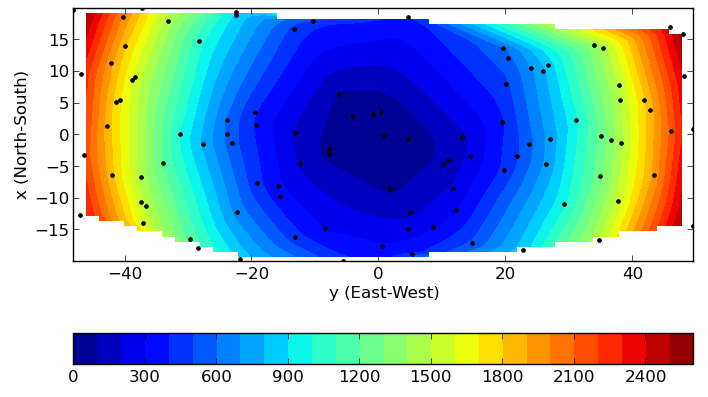
\includegraphics[width=\textwidth]{figures/paper1/gridding_plotting_contourf}
    \caption{
    Example of 1) generating a random scatter of points (black dots),
    2) using that to make synthetic data, and
    3) automatically gridding and plotting the data using a
    Fatiando a Terra wrapper for the Matplotlib ``contourf``
    function.
    }
    \label{fig:contourf}
\end{figure}


Notice that, in the calls to \texttt{mpl.contourf} and
\texttt{mpl.plot}, the x- and y-axis are switched. That is because it is
common practice in geophysics for x to point North and y to point East.

Map projections in Matplotlib are handled by the
\href{http://matplotlib.org/basemap}{Basemap toolkit}. The
\texttt{fatiando.vis.mpl} module also provides helper functions to
automate the use of this toolkit. The \texttt{fatiando.vis.mpl.basemap}
function automates the creation of the \texttt{Basemap} objects with
common parameters. This object can then be passed to the
\texttt{contourf}, \texttt{contour} and \texttt{pcolor} functions in
\texttt{fatiando.vis.mpl} and they will automatically plot using the
given projection (Figure~\ref{fig:basemap}):

\begin{verbatim}
mpl.figure()
bm = mpl.basemap(area, projection='robin')
bm.drawmapboundary()
bm.drawcoastlines()
mpl.contourf(x, y, data, shape=(50, 50), levels=30,
    interp=True, basemap=bm)
mpl.colorbar(orientation='horizontal')
mpl.show()
\end{verbatim}

\begin{figure}
    \centering
    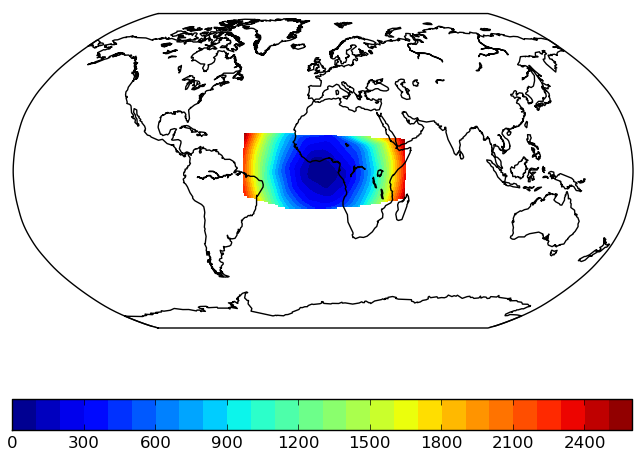
\includegraphics[width=\textwidth]{figures/paper1/gridding_plotting_basemap}
    \caption{
        Example of map plotting with the Robinson projection using the
        Matplotlib Basemap toolkit.
    }
    \label{fig:basemap}
\end{figure}



\section{Meshes and 3D plotting}

The representation of 2D and 3D geometric elements is handled by the
classes in the \texttt{fatiando.mesher} module. Geometric elements in
Fatiando a Terra can be assigned physical property values, like density,
magnetization, seismic wave velocity, impedance, etc. This is done
through a \texttt{props} dictionary whose keys are the name of the
physical property and values are the corresponding values in SI units:

\begin{verbatim}
from fatiando import mesher
model = [
    mesher.Prism(5, 8, 3, 7, 1, 7,
        props={'density':200}),
    mesher.Prism(1, 2, 4, 5, 1, 2,
        props={'density':1000})]
\end{verbatim}

The \texttt{fatiando.vis.myv} module contains functions to automate 3D plotting
using Mayavi \citep{ramachandran2011}. The \texttt{mayavi.mlab} interface
requires geometric elements to be formatted as TVTK objects. Thus, plotting
functions in \texttt{fatiando.vis.myv} automatically create TVTK
representations of \texttt{fatiando.mesher} objects and plot them using a
suitable function of \texttt{mayavi.mlab}. Also included are utility functions
for drawing axes, walls on the figure bounding box, etc. For example, the
\texttt{fatiando.vis.myv.figure} function creates a figure and rotates it so
that the z-axis points down, as is standard in geophysics. The following
example shows how to plot the 3D right rectangular prism model that we created
previously (Figure~\ref{fig:twoprisms}):

\begin{verbatim}
from fatiando.vis import myv
bounds = [0, 10, 0, 10, 0, 10]
myv.figure()
myv.prisms(model, 'density')
myv.axes(myv.outline(bounds))
myv.wall_bottom(bounds)
myv.wall_north(bounds)
myv.show()
\end{verbatim}

\begin{figure}
    \centering
    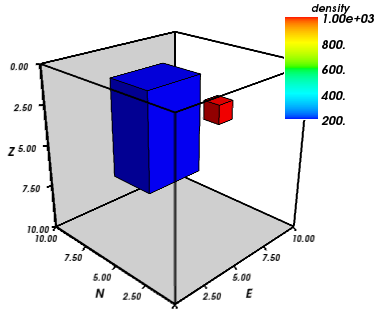
\includegraphics[width=0.7\textwidth]{figures/paper1/meshes_3dplotting_2prisms}
    \caption{
        Example of plotting a list of right rectangular prisms in Mayavi.
    }
    \label{fig:twoprisms}
\end{figure}

The \texttt{fatiando.mesher} module also contains classes for
collections of elements (e.g., meshes). A good example is the
\texttt{PrismMesh} class that represents a structured mesh of right
rectangular prisms. This class behaves as a list of
\texttt{fatiando.mesher.Prism} objects and can be passed to functions
that ask for a list of prisms, like \texttt{fatiando.vis.myv.prisms}.
Physical properties can be assigned to the mesh using the
\texttt{addprop} method (Figure~\ref{fig:mesh}):

\begin{verbatim}
mesh = mesher.PrismMesh(bounds, shape=(3, 3, 3))
mesh.addprop('density', range(mesh.size))
myv.figure()
myv.prisms(mesh, 'density')
myv.axes(myv.outline(bounds))
myv.show()
\end{verbatim}

\begin{figure}
    \centering
    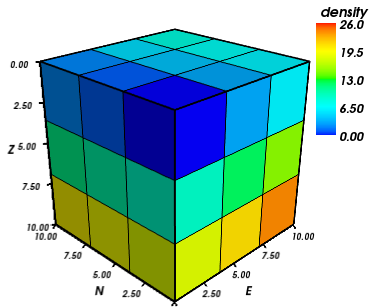
\includegraphics[width=0.7\textwidth]{figures/paper1/meshes_3dplotting_mesh}
    \caption{
        Example of generating and visualizing a structured prism mesh.
    }
    \label{fig:mesh}
\end{figure}

Often times the mesh is used to make a detailed model of an irregular
region of the Earth's surface. In such cases, it is necessary to
consider the topography of the region. The \texttt{PrismMesh} class has
a \texttt{carvetopo} method that masks the prisms that fall above the
topography. The example below illustrates this functionality using
synthetic topography (Figure~\ref{fig:meshtopo}):

\begin{verbatim}
from fatiando import utils
x, y = gridder.regular(bounds[:4], (50, 50))
heights = -5 + 5*utils.gaussian2d(x, y, 10, 5,
    x0=10, y0=10)
mesh = mesher.PrismMesh(bounds, (20, 20, 20))
mesh.addprop('density', range(mesh.size))
mesh.carvetopo(x, y, heights)
myv.figure()
myv.prisms(mesh, 'density')
myv.axes(myv.outline(bounds))
myv.wall_north(bounds)
myv.show()
\end{verbatim}

\begin{figure}
    \centering
    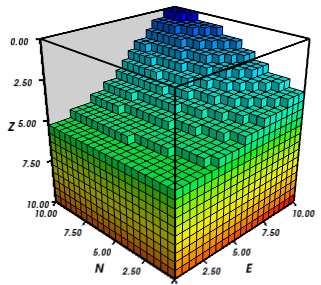
\includegraphics[width=0.7\textwidth]{figures/paper1/meshes_3dplotting_meshtopo}
    \caption{
        Example of generating and visualizing a prism mesh with masked
        topography.
    }
    \label{fig:meshtopo}
\end{figure}

When modeling involves the whole Earth, or a large area of it, the
geophysicist needs to take into account the Earth's curvature. In such
cases, rectangular prisms are inadequate for modeling and tesseroids
(e.g., spherical prisms) are better suited. The
\texttt{fatiando.vis.myv} module contains auxiliary functions to plot
along with tesseroids: an Earth-sized sphere, meridians and parallels,
as well as continental borders (Figure~\ref{fig:tesseroid}):

\begin{verbatim}
model = [
    mesher.Tesseroid(-60, -55, -30, -27, 500000, 0,
        props={'density':200}),
    mesher.Tesseroid(-66, -55, -20, -10, 300000, 0,
        props={'density':-100})]
fig = myv.figure(zdown=False)
myv.tesseroids(model, 'density')
myv.continents(linewidth=2)
myv.earth(opacity=1)
myv.meridians(range(0, 360, 45), opacity=0.2)
myv.parallels(range(-90, 90, 45), opacity=0.2)
# Rotate the camera to get a good view
scene = fig.scene
scene.camera.position = [21199620.406122234,
    -12390254.839673528, -14693312.866768979]
scene.camera.focal_point = [-535799.97230670298,
    -774902.33205294283, 826712.82283183688]
scene.camera.view_angle = 19.199999999999996
scene.camera.view_up = [0.33256519487680014,
    -0.47008782429014295, 0.81756824095039038]
scene.camera.clipping_range = [7009580.0037488714,
    55829873.658824757]
scene.camera.compute_view_plane_normal()
scene.render()
myv.show()
\end{verbatim}

\begin{figure}
    \centering
    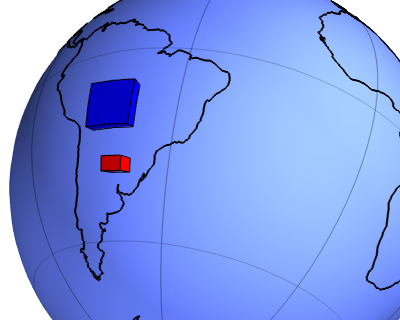
\includegraphics[width=0.7\textwidth]{figures/paper1/meshes_3dplotting_tesseroid}
    \caption{
        Example of creating a tesseroid (spherical prism) model and visualizing
        it in Mayavi.
    }
    \label{fig:tesseroid}
\end{figure}




\section{Forward modeling}

In geophysics, the term ``forward modeling'' is used to describe the
process of generating synthetic data from a given Earth model.
Conversely, geophysical inversion is the process of estimating Earth
model parameters from observed data.

The Fatiando a Terra packages have separate modules for forward modeling
and inversion algorithms. The forward modeling functions usually take as
arguments geometric elements from \texttt{fatiando.mesher} with assigned
physical properties and return the synthetic data. For example, the
module \texttt{fatiando.gravmag.tesseroid} is a Python implementation of
the program Tesseroids (\url{http://leouieda.github.io/tesseroids}) and
calculates the gravitational fields of tesseroids (e.g., spherical
prisms). The following example shows how to calculate the gravity
anomaly of the tesseroid model generated in the previous section
(Figure~\ref{fig:tesseroidgrav}):

\begin{verbatim}
from fatiando import gravmag
area = [-80, -30, -40, 10]
shape = (50, 50)
lons, lats, heights = gridder.regular(area, shape,
    z=2500000)
gz = gravmag.tesseroid.gz(lons, lats, heights, model)
mpl.figure()
bm = mpl.basemap(area, 'ortho')
bm.drawcoastlines()
bm.drawmapboundary()
bm.bluemarble()
mpl.title('Gravity anomaly (mGal)')
mpl.contourf(lons, lats, gz, shape, 30, basemap=bm)
mpl.colorbar()
mpl.show()
\end{verbatim}

\begin{figure}
    \centering
    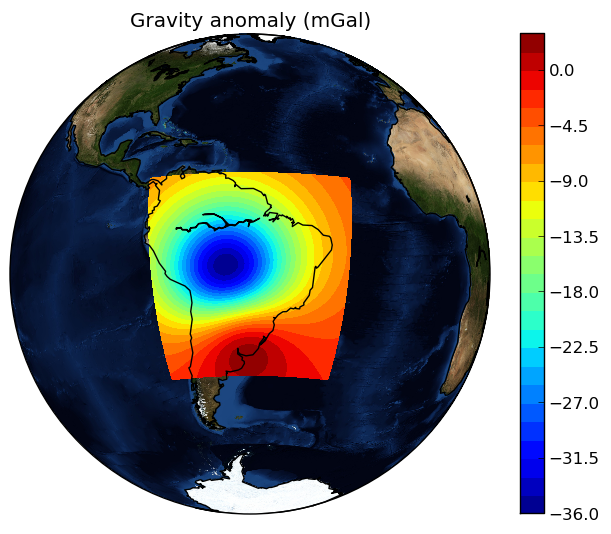
\includegraphics[width=0.7\textwidth]{figures/paper1/gravmag_tesseroid_data}
    \caption{
        Example of forward modeling the gravity anomaly using the tesseroid
        model shown in Figure~\ref{fig:tesseroid}.
    }
    \label{fig:tesseroidgrav}
\end{figure}

The module \texttt{fatiando.gravmag.polyprism} implements the method of
\citet{plouff1976} to forward model the gravity fields of a 3D right polygonal
prism. The following code sample shows how to interactively generate a
polygonal prism model and calculate its gravity anomaly
(Figures~\ref{fig:drawing} and \ref{fig:polyprism}):

\begin{verbatim}
# Draw a polygon and make a polygonal prism
bounds = [-1000, 1000, -1000, 1000, 0, 1000]
area = bounds[:4]
mpl.figure()
mpl.axis('scaled')
vertices = mpl.draw_polygon(area, mpl.gca(),
    xy2ne=True)
model = [mesher.PolygonalPrism(vertices, z1=0,
    z2=500, props={'density':500})]
# Calculate the gravity anomaly
shape = (100, 100)
x, y, z = gridder.scatter(area, 300, z=-1)
gz = gravmag.polyprism.gz(x, y, z, model)
mpl.figure()
mpl.axis('scaled')
mpl.title("Gravity anomaly (mGal)")
mpl.contourf(y, x, gz, shape=(50, 50),
    levels=30, interp=True)
mpl.colorbar()
mpl.polygon(model[0], '.-k', xy2ne=True)
mpl.set_area(area)
mpl.m2km()
mpl.show()
myv.figure()
myv.polyprisms(model, 'density')
myv.axes(myv.outline(bounds),
        ranges=[i*0.001 for i in bounds])
myv.wall_north(bounds)
myv.wall_bottom(bounds)
myv.show()
\end{verbatim}

\begin{figure}
    \centering
    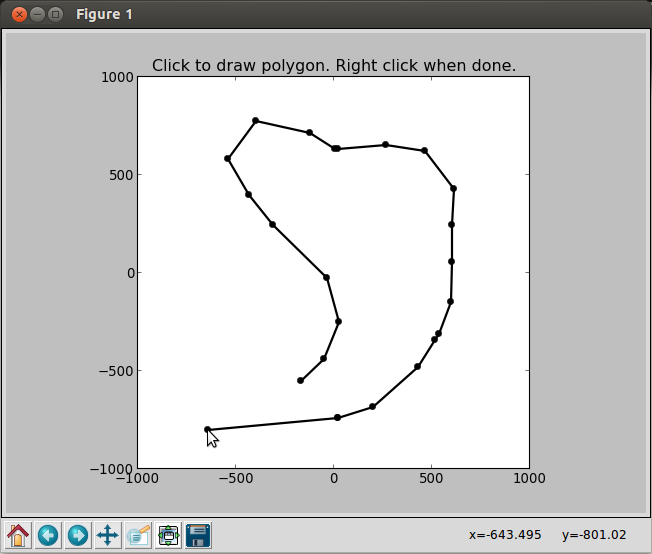
\includegraphics[width=0.7\textwidth]{figures/paper1/forward_modeling_polyprism_drawing}
    \caption{
        Screen-shot of interactively drawing the contour of a 3D polygonal
        prism, as viewed from above.
    }
    \label{fig:drawing}
\end{figure}

\begin{figure}
    \centering
    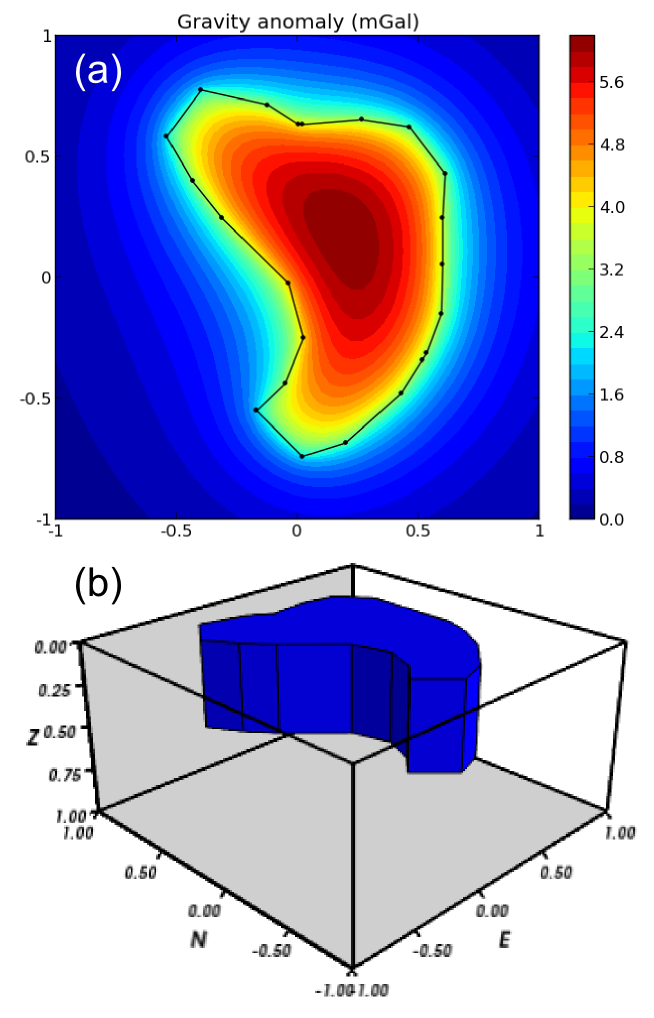
\includegraphics[width=0.5\textwidth]{figures/paper1/forward_modeling_polyprism}
    \caption{
        Example of forward modeling the gravity anomaly of a 3D polygonal
        prism.
        a) forward modeled gravity anomaly.
        b) 3D plot of the polygonal prism.
    }
    \label{fig:polyprism}
\end{figure}




\section{Gravity and magnetic methods}

Geophysics uses anomalies in the gravitational and magnetic fields
generated by density and magnetization contrasts within the Earth to
investigate the inner Earth structure. The Fatiando a Terra 0.1 release
has been focused on gravity and magnetic methods. Therefore, the
\texttt{fatiando.gravmag} package contains more advanced and
state-of-the-art algorithms than the other packages.

The module \texttt{fatiando.gravmag.imaging} implements the imaging methods
described in \citet{fedi2012}. These methods aim to produce an image of the
geologic source from the observed gravity or magnetic data. The following code
sample uses the ``sandwich model'' method \citep{pedersen1991} to image the
polygonal prism, produced in the previous section, based on its gravity anomaly
(Figure~\ref{fig:imaging}):

\begin{verbatim}
estimate = gravmag.imaging.sandwich(x, y, z, gz,
    shape, zmin=0, zmax=1000, nlayers=20, power=0.2)
body = mesher.vfilter(1.3*10**8, 1.7*10**8,
    'density', estimate)
myv.figure()
myv.prisms(body, 'density', edges=False)
p = myv.polyprisms(model, 'density',
    style='wireframe', linewidth=4)
p.actor.mapper.scalar_visibility = False
p.actor.property.color = (0, 0, 0)
myv.axes(myv.outline(bounds),
    ranges=[i*0.001 for i in bounds])
myv.wall_north(bounds)
myv.wall_bottom(bounds)
myv.show()
\end{verbatim}

\begin{figure}
    \centering
    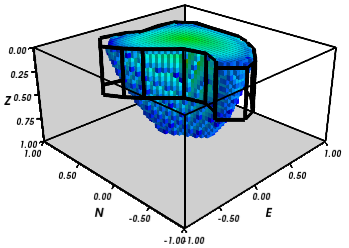
\includegraphics[width=0.7\textwidth]{figures/paper1/gravmag_imaging}
    \caption{
        Example of using the "sandwich model" imaging method to recover a 3D
        image of a geologic body based on its gravity anomaly. The colored
        blocks are a cutoff of the imaged body. The black contours are the true
        source of the gravity anomaly.
    }
    \label{fig:imaging}
\end{figure}

Also implemented in Fatiando a Terra are some recent developments in
gravity and magnetic inversion methods. The method of ``planting
anomalous densities'' by \citet{uieda2012} is implemented in the
\texttt{fatiando.gravmag.harvester} module. In contrast to imaging
methods, this is an inversion method, i.e., it estimates a physical
property distribution (density in the case of gravity data) that fits
the observed data. This particular method requires the user to specify a
``seed'' (Figure~\ref{fig:seed}) around which the estimated density
distribution grows (Figure~\ref{fig:harvester}):

\begin{verbatim}
# Make a mesh and a seed
mesh = mesher.PrismMesh(bounds, (15, 30, 30))
seeds = gravmag.harvester.sow(
    [[200, 300, 100, {'density':500}]],
    mesh)
myv.figure()
myv.prisms([mesh[s.i] for s in seeds])
p = myv.polyprisms(model, 'density',
    style='wireframe', linewidth=4)
p.actor.mapper.scalar_visibility = False
p.actor.property.color = (0, 0, 0)
myv.axes(myv.outline(bounds),
    ranges=[i*0.001 for i in bounds])
myv.wall_north(bounds)
myv.wall_bottom(bounds)
myv.show()
# Now perform the inversion
data = [gravmag.harvester.Gz(x, y, z, gz)]
estimate = gravmag.harvester.harvest(data, seeds,
    mesh, compactness=0.1, threshold=0.0001)[0]
mesh.addprop('density', estimate['density'])
body = mesher.vremove(0, 'density', mesh)
myv.figure()
myv.prisms(body, 'density')
p = myv.polyprisms(model, 'density',
    style='wireframe', linewidth=4)
p.actor.mapper.scalar_visibility = False
p.actor.property.color = (0, 0, 0)
myv.axes(myv.outline(bounds),
    ranges=[i*0.001 for i in bounds])
myv.wall_north(bounds)
myv.wall_bottom(bounds)
myv.show()
\end{verbatim}

\begin{figure}
    \centering
    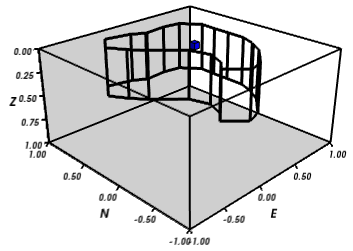
\includegraphics[width=0.7\textwidth]{figures/paper1/gravmag_harvester_seed}
    \caption{
        The small blue prism is the seed used by
        \texttt{fatiando.gravmag.harvester} to perform the inversion of a
        gravity anomaly. The black contours are the true source of the gravity
        anomaly.
    }
    \label{fig:seed}
\end{figure}

\begin{figure}
    \centering
    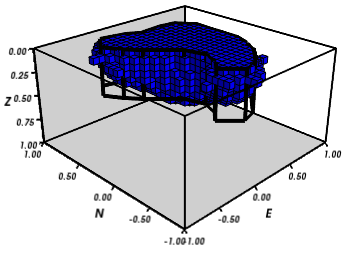
\includegraphics[width=0.7\textwidth]{figures/paper1/gravmag_harvester}
    \caption{
        The blue prisms are the result of a gravity inversion using module
        \texttt{fatiando.gravmag.harvester}. The black contours are the true
        source of the gravity anomaly. Notice how the inversion was able to
        recover the approximate geometry of the true source.
    }
    \label{fig:harvester}
\end{figure}




\section{A toy seismic tomography}

The following example uses module \texttt{fatiando.seismic.srtomo} to
perform a simplified 2D tomography on synthetic seismic wave travel-time
data. To generate the travel-times we used a seismic wave velocity model
constructed from an image file. The colors of the image are converted to
gray-scale and the intensity is mapped to seismic wave velocity by the
\texttt{img2prop} method of the \texttt{fatiando.mesher.SquareMesh}
class. This model (Figure~\ref{fig:tomo}) is then used to calculate the
travel-times between a random set of earthquake locations and seismic
receivers (seismometers):

\begin{verbatim}
import urllib
from fatiando import mesher, utils, seismic
from fatiando.vis import mpl
area = (0, 500000, 0, 500000)
shape = (30, 30)
model = mesher.SquareMesh(area, shape)
link = '/'.join(["http://fatiando.readthedocs.org",
    "en/Version0.1/_static/logo.png"])
urllib.urlretrieve(link, 'model.png')
model.img2prop('model.png', 4000, 10000, 'vp')
quake_locations = utils.random_points(area, 40)
receiver_locations = utils.circular_points(area, 20,
    random=True)
quakes, receivers = utils.connect_points(
    quake_locations, receiver_locations)
traveltimes = seismic.ttime2d.straight(model, 'vp',
    quakes, receivers)
noisy = utils.contaminate(traveltimes, 0.001,
    percent=True)
\end{verbatim}

Now the noise-corrupted synthetic travel-times can be used in our
simplified tomography:

\begin{verbatim}
mesh = mesher.SquareMesh(area, shape)
slowness, residuals = seismic.srtomo.run(noisy,
    quakes, receivers, mesh, smooth=10**6)
velocity = seismic.srtomo.slowness2vel(slowness)
mesh.addprop('vp', velocity)
# Make the plots
mpl.figure(figsize=(9, 7))
mpl.subplots_adjust(top=0.95, bottom=0.05,
    left=0.05, right=0.95)
mpl.subplot(2, 2, 1)
mpl.title('Velocity model (m/s)')
mpl.axis('scaled')
mpl.squaremesh(model, prop='vp', cmap=mpl.cm.seismic)
mpl.colorbar(pad=0.01)
mpl.points(quakes, '*y', label="Sources")
mpl.points(receivers, '^g', label="Receivers")
mpl.m2km()
mpl.subplot(2, 2, 2)
mpl.title('Ray paths')
mpl.axis('scaled')
mpl.squaremesh(model, prop='vp', cmap=mpl.cm.seismic)
mpl.colorbar(pad=0.01)
mpl.paths(quakes, receivers)
mpl.points(quakes, '*y', label="Sources")
mpl.points(receivers, '^g', label="Receivers")
mpl.m2km()
mpl.subplot(2, 2, 3)
mpl.title('Estimated velocity (m/s)')
mpl.axis('scaled')
mpl.squaremesh(mesh, prop='vp', cmap=mpl.cm.seismic,
    vmin=4000, vmax=10000)
mpl.colorbar(pad=0.01)
mpl.m2km()
mpl.subplot(2, 2, 4)
mpl.title('Residuals (s)')
mpl.hist(residuals, bins=10)
mpl.show()
\end{verbatim}

Even though the implementation in \texttt{fatiando.seismic.srtomo} is greatly
simplified and not usable in real tomography problems, the result in
Figure~\ref{fig:tomo} illustrates interesting inverse problem concepts.  Notice
how the estimated velocity is blurred in the corners where no rays pass
through. This is because the data (travel-times) provide no information about
the velocity in those areas. Areas like those constitute the null space of the
inverse problem \citep{menke1984}, where any velocity value estimated will
provide an equal fit to the data.  Thus, the tomography problem requires the
use of prior information in the form of regularization. Most commonly used in
tomography problems is the Tikhonov first-order regularization, e.g., a
smoothness constraint \citep{menke1984}. The amount of smoothness imposed on
the solution is controlled by the \texttt{smooth} argument of function
\texttt{fatiando.seismic.srtomo.run}. That is how we are able to estimate a
unique and stable solution and why the result is specially smoothed where there
are no rays.



\begin{figure}
    \centering
    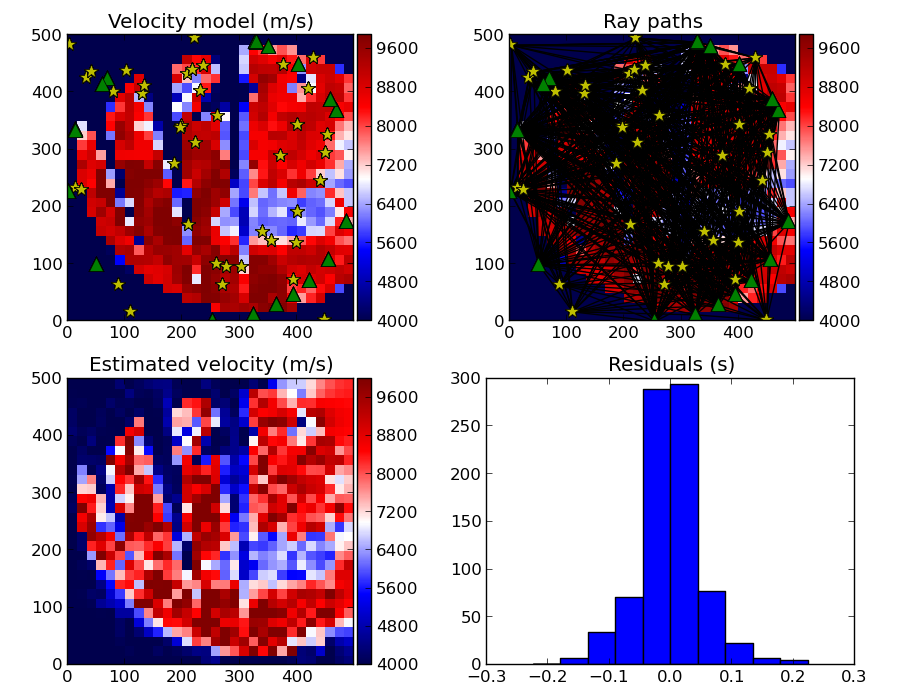
\includegraphics[width=\textwidth]{figures/paper1/seismic_tomo}
    \caption{
        Example run of a simplified 2D tomography. The top-left panel shows the
        true velocity model with the locations of earthquakes (yellow stars)
        and receivers (green triangles). The top-right panel shows the
        ray-paths between earthquakes and receivers. The bottom-left panel is
        the velocity estimated by the tomography. The bottom-right panel is a
        histogram of the travel-time residuals of the tomography. Notice how
        the majority of residuals are close to 0 s, indicating a good fit to
        the data.
    }
    \label{fig:tomo}
\end{figure}




\section{Conclusion}

The Fatiando a Terra package provides an API to develop modeling
algorithms for a variety of geophysical methods. The current version
(0.1) has a few state-of-the-art gravity and magnetic modeling and
inversion algorithms. There are also toy problems in gravity, seismics
and seismology that are useful for teaching basic concepts of
geophysics, modeling, and inverse problems.

Fatiando a Terra enables quick prototyping of new algorithms because of
the collection of fast forward modeling routines and the simple syntax
and high level of the Python language. After prototyping, the
performance bottlenecks of these algorithms can be easily diagnosed
using the advanced profiling tools available in the Python language.
Optimization of only small components of code can be done without loss
of flexibility using the Cython language \citep{behnel2011}.

The biggest challenge that Fatiando a Terra faces in the near future is
the development of a user and, consequently, a developer community. This
is a key part for the survival of any open-source project.




\section{Acknowledgments}

The authors were supported by a scholarship (L. Uieda) from Coordenação de
Aperfeiçoamento de Pessoal de Nível Superior (CAPES), a scholarship (V.C.
Oliveira Jr) from Conselho Nacional de Desenvolvimento Científico e Tecnológico
(CNPq), and a fellowship (V.C.F. Barbosa) from CNPq.  Additional support was
provided by the Brazilian agencies CNPq (grant 471693/2011-1) and FAPERJ (grant
E-26/103.175/2011).

\chapter{Tesseroids: forward modeling gravitational fields in spherical coordinates}
\label{chap:tesseroids}


This chapter has been submitted for publication in the journal Geophysics in
collaboration with Dr. Carla Braitenberg of the University of Trieste, Italy.

\section{Abstract}

We present the open-source software \emph{Tesseroids},
a set of command-line programs to perform the forward modeling
of gravitational fields in spherical coordinates.
The software is implemented in the C programming language and uses tesseroids
(spherical prisms) for the discretization of the subsurface mass distribution.
The gravitational fields of tesseroids are calculated numerically using
the Gauss-Legendre Quadrature (GLQ).
We have improved upon an adaptive discretization algorithm
to guarantee the accuracy of the GLQ integration.
Our implementation of adaptive discretization
uses a ``stack'' based algorithm
instead of recursion to achieve
more control over execution errors and corner cases.
The algorithm is controlled by
a scalar value called the distance-size ratio ($D$)
that determines the accuracy of the integration as well as
the computation time.
We determined optimal values of $D$
for the gravitational potential, gravitational acceleration,
and gravity gradient tensor
by comparing the computed tesseroids effects
with those of a homogeneous spherical shell.
The values required for a maximum relative error of 0.1\% of the shell effects
are $D = 1$ for the gravitational potential, $D = 1.5$ for the gravitational
acceleration, and $D = 8$ for the gravity gradients.
Contrary to previous assumptions,
our results show that the potential and its first and second derivatives
require different values of $D$ to achieve the same accuracy.
These values were incorporated as defaults in the software.


%%%%%%%%%%%%%%%%%%%%%%%%%%%%%%%%%%%%%%%%%%%%%%%%%%%%%%%%%%%%%%%%%%%%%%%%%%%%%%
\section{Introduction}


Satellite missions dedicated to measuring the Earth's gravity field
(like CHAMP, GRACE, and GOCE)
have provided geophysicists with almost uniform and global data coverage.
These new data have enabled interpretations on regional and global scales
\citep[e.g.][]{reguzzoni2013,braitenberg2015}.
Modeling at such scales requires taking into account the curvature of the
Earth and calculating gravity gradients as well as the traditional
gravitational acceleration.
A common approach to achieve this is
to discretize the Earth into tesseroids (Figure~\ref{fig:p2-tesseroid})
instead of rectangular prisms.
An analytical solution exists when the computation point is along
the polar axis and the tesseroid is extended into a spherical cap
\citep{lafehr1991a, mikuska2006, grombein2013}.
For more general cases,
the integral formula for the gravitational effects of a tesseroid
must be solved numerically.
Approaches to this numerical integration include
Taylor series expansion \citep{heck2007, grombein2013}
and the Gauss-Legendre Quadrature \citep{asgharzadeh2007}.
Taylor series expansion produces accurate results at low latitudes but
presents a decrease in accuracy towards the polar regions.
This is attributed to tesseroids degenerating into an approximately triangular
shape at the poles.
The Gauss-Legendre Quadrature (GLQ) integration consists in approximating
the volume integral by a weighted sum of the effect of point masses.
An advantage of the GLQ approach is that it can be
controlled by the number of point masses used.
The larger the number of point masses,
the better the accuracy of GLQ integration.
A disadvantage is the increased computation time as the number of
point masses increases.
Thus, there is a trade-off between accuracy and computation time.
This is a common theme in numerical methods.
\citet{wild-pfeiffer2008} investigated the use of different mass elements,
including tesseroids, to compute the gravitational effects of topographic
masses.
The author concludes that using tesseroids with GLQ integration gives the best
results for near-zone computations.
However, the question of how to determine the optimal parameters for GLQ
integration remained open.


Previous work by \citet{ku1977} investigated the use of the GLQ
in gravity forward modeling.
\citet{ku1977} numerically integrated the vertical component of the
gravitational acceleration of right rectangular prisms.
The author suggested that the accuracy of the GLQ integration depends on
the ratio between distance to the computation point and the distance between
adjacent point masses.
Based on this, \citet{ku1977} proposed an empirical criterion that
the distance between point masses should be greater than
the distance to the computation point.
\citet{asgharzadeh2007} used  this criterion for the GLQ integration of
the gravity gradient tensor of tesseroids.
To our knowledge, an analysis of how well this ad hoc criteria of
\citet{ku1977} works for gravity gradient components or for tesseroids
has never been done before.
There has also been no attempt to quantify the error committed in the GLQ
integration when applying the criteria of \citet{ku1977}.

\citet{li2011} devised an algorithm to automatically enforce the criteria of
\citet{ku1977}.
Their algorithm divides the tesseroid into smaller ones instead of increasing
the number of point masses per tesseroid.
A tesseroid is divided if the minimum distance to the computation point
is smaller than the largest dimension of the tesseroid.
This division is repeated recursively until all tesseroids obey the criterion.
Then, GLQ integration is performed for each of the smaller tesseroids
using the specified number of point masses.
The advantage of this adaptive discretization over
increasing the number of points masses is that the
total distribution of point masses will be greater
only close to the computation point.
This makes the adaptive discretization more computationally efficient.

\citet{grombein2013} developed optimized formula for the gravitational fields
of tesseroids using Cartesian integral kernels.
These formulas are faster to compute and do not have singularities at the poles
like their spherical counterparts.
The Cartesian formulae are numerically integrated using a Taylor series
expansion as per \citet{heck2007}.
\citet{grombein2013} use a near-zone separation to mitigate the increased error
at high latitudes.
In the so called ``near-zone'' of the computation point they use a finer
discretization composed by smaller tesseroids.
This is accomplished by dividing the tesseroids along their horizontal
dimensions.
However, the determination of an optimal size of the near-zone remains an
open question \citep{grombein2013}.

We have implemented a modified version of the adaptive discretion of
\citet{li2011} into the open-source software package \emph{Tesseroids}.
The software uses the Cartesian formula of \citet{grombein2013} for improved
performance and robustness.
Previous versions of the software have been used by, e.g.,
\citet{alvarez2012, bouman2013, bouman2013a, mariani2013, braitenberg2015,
braitenberg2011, fullea2015a}.

This article describes the software design and the implementation
of our modified adaptive discretization algorithm.
We also present a numerical investigation of the error committed
in the computations.
These results allow us to calibrate the adaptive discretization algorithm
separately for the gravitational potential, gravitational acceleration,
as well as the gravity gradient tensor components.


%%%%%%%%%%%%%%%%%%%%%%%%%%%%%%%%%%%%%%%%%%%%%%%%%%%%%%%%%%%%%%%%%%%%%%%%%%%%%%
\section{Theory}


\begin{figure}
    \centering
    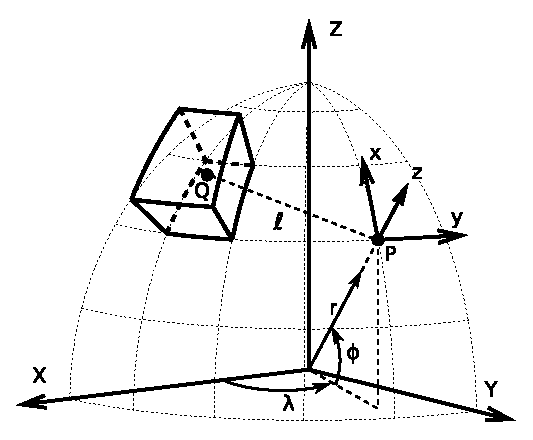
\includegraphics{figures/paper2/tesseroid}
    \caption{
        View of a tesseroid,
        the integration point $Q$ inside the tesseroid,
        a geocentric coordinate system $(X, Y, Z)$,
        the computation $P$ and it's local coordinate system $(x, y, z)$.
        $r$, $\phi$, $\lambda$ are
        the radius, latitude, and longitude, respectively, of point $P$,
        and $\ell$ is the Cartesian distance between $P$ and $Q$.
    }
    \label{fig:p2-tesseroid}
\end{figure}

A tesseroid is a mass element defined in geocentric spherical
coordinates
(Figure~\ref{fig:p2-tesseroid}).
It is bounded by two meridians, two parallels, and two concentric circles.
The gravitational fields of a tesseroid at a point $P = (r,\phi,\lambda)$
are determined with respect to the local North-oriented coordinate system at
P (x, y, z in Figure~\ref{fig:p2-tesseroid}).
\citet{grombein2013} formulated Cartesian kernels for the volume integrals
that define the tesseroid gravitational potential, gravitational acceleration,
and Marussi tensor, respectively,

\begin{equation}
    V(r,\phi,\lambda) = G \rho
        \int\limits_{\lambda_1}^{\lambda_2}
        \int\limits_{\phi_1}^{\phi_2}
        \int\limits_{r_1}^{r_2}
        \frac{1}{\ell}
        \kappa\  dr^\prime d\phi^\prime d\lambda^\prime,
    \label{eq:p2-tesspot}
\end{equation}
\begin{equation}
    g_{\alpha}(r,\phi,\lambda) = G \rho
        \int\limits_{\lambda_1}^{\lambda_2}
        \int\limits_{\phi_1}^{\phi_2}
        \int\limits_{r_1}^{r_2}
        \frac{\Delta_\alpha}{\ell^3}
        \kappa\ dr^\prime d\phi^\prime d\lambda^\prime,
    \label{eq:p2-tessgrav}
\end{equation}
\noindent
and
\begin{equation}
    g_{\alpha\beta}(r,\phi,\lambda) = G \rho
        \int\limits_{\lambda_1}^{\lambda_2}
        \int\limits_{\phi_1}^{\phi_2}
        \int\limits_{r_1}^{r_2}
        I_{\alpha\beta}
        \ \kappa\ dr^\prime d\phi^\prime d\lambda^\prime ,
    \label{eq:p2-tesstensor}
\end{equation}
\begin{equation}
    I_{\alpha\beta} =
    \left(
        \frac{3\Delta_{\alpha} \Delta_{\beta}}{\ell^5} -
        \frac{\delta_{\alpha\beta}}{\ell^3}
    \right) ,
    \label{eq:p2-tesstensorkernel}
\end{equation}

\noindent
where $\alpha, \beta \in \{x, y, z\}$,
$\rho$ is the density,
$G = 6.674\times10^{-11}\ m^3kg^{-1}s^{-1}$ is the gravitational constant,
$\delta_{\alpha\beta}$ is Kronecker's delta
($\delta_{\alpha\beta} = 1$ if $\alpha = \beta$
and $\delta_{\alpha\beta} = 0$ if $\alpha \neq \beta$),
and

\begin{equation}
    \Delta_x = r^\prime(\cos\phi\sin\phi^\prime - \sin\phi\cos\phi^\prime
               \cos(\lambda^\prime - \lambda)),
\end{equation}
\begin{equation}
    \Delta_y = r^\prime \cos \phi^\prime \sin(\lambda^\prime - \lambda),
\end{equation}
\begin{equation}
    \Delta_z = r^\prime \cos \psi - r,
\end{equation}
\begin{equation}
    \kappa = {r^\prime}^2 \cos \phi^\prime,
\end{equation}
\begin{equation}
    \ell = \sqrt{{r^\prime}^2 + r^2 - 2 r^\prime r \cos \psi},
\end{equation}
\begin{equation}
    \cos\psi = \sin\phi\sin\phi^\prime + \cos\phi\cos\phi^\prime
                 \cos(\lambda^\prime - \lambda).
\end{equation}

We will follow \citet{asgharzadeh2007} and perform the numerical integration
using the Gauss-Legendre Quadrature (GLQ).
The GLQ consists in approximating the integral by a weighted sum of the
integration kernel \citep{hildebrand1987},

\begin{equation}
    \int\limits_a^b f(x) dx \approx
    \frac{b-a}{2}\sum\limits_{i=1}^N W_i f(x_i),
    \label{eq:p2-glq1d}
\end{equation}

\noindent
in which $N$ is the order of the quadrature,
i.e. the number of points used in the GLQ.
The points $x_i$ are called the quadrature nodes.
They are the roots of the $N^{th}$ order Legendre polynomial $P_N(x)$.
For a second order polynomial ($P_2(x)$),
the roots are $x = \pm 0.577350269$.
Roots for larger order polynomials
can be determined by a root finder algorithm.
Roots of Legendre polynomials
will be within the range $[-1, 1]$.
Before being used for GLQ integration,
the roots must be scaled to the integration limits $[a, b]$ using

\begin{equation}
    x^{scaled}_i = \frac{b - a}{2} x_i + \frac{b + a}{2}.
    \label{eq:p2-glq_scaling}
\end{equation}

The weights of the GLQ are given by \citep{hildebrand1987},

\begin{equation}
    W_i = \frac{2}{(1 - x_i^2)(P^\prime_N(x_i))^2}.
    \label{eq:p2-glq_weights}
\end{equation}

\noindent
The values of $P_N(x)$ and its first derivative $P^\prime_N(x)$
can be calculated with recursive relations.

The Gauss-Legendre Quadrature for three-dimensional volume integrals,
like equations~\ref{eq:p2-tesspot}-\ref{eq:p2-tesstensor},
becomes \citep{asgharzadeh2007}

\begin{equation}
    \iiint\limits_{\Omega}
    f(r^\prime, \lambda^\prime, \phi^\prime)
    d\Omega
    \approx
    A
    \sum\limits_{i=1}^{N^r}
    \sum\limits_{j=1}^{N^\phi}
    \sum\limits_{k=1}^{N^\lambda}
    W_i^r W_j^\phi W_k^\lambda
    f(r_i, \phi_j, \lambda_k),
    \label{eq:p2-glq3d}
\end{equation}

\noindent
where

\begin{equation}
    A = \frac{(\lambda_2 - \lambda_1)(\phi_2 - \phi_1)(r_2 - r_1)}{8}.
\end{equation}

Comparing equation~\ref{eq:p2-glq3d} with
equations~\ref{eq:p2-tesspot}-\ref{eq:p2-tesstensor},
we see that $f(r_i, \phi_j, \lambda_k)$ is the effect of a point
mass located on the quadrature nodes.
Thus, it can be said that the GLQ integration
approximates the volume integrals  by a
weighted sum of point mass effects.

The accuracy of the integration
depends on the number of point masses used in the summation.
\citet{ku1977} showed that it also depends on the ratio between
the distance to the computation point and the distance between adjacent nodes.
Figure~\ref{fig:p2-glqerrorsample}
illustrates this effect on the $g_{xy}$ gravity gradient component.
The $g_{xy}$ component was produced by a
$7^\circ \times 7^\circ \times 20\ km$ tesseroid
with $2.67\ g.cm^{-3}$ density
and top at $z=0\ km$.
The maps were calculated on a regular grid
with $100\times100$ points.
Figure~\ref{fig:p2-glqerrorsample}a shows the $g_{xy}$ component
calculated at 400 km height using
GLQ with order two ($2 \times 2 \times 2 = 8$ point masses).
Figure~\ref{fig:p2-glqerrorsample}b shows $g_{xy}$ computed with order two
GLQ as well but at 150 km height.
Notice that the computed effect is concentrated around each point mass
of the GLQ (black dots) and does not resemble the effect of a tesseroid.
\citet{ku1977} determined an ad hoc criterion that the distance between
point masses (quadrature nodes) should be smaller than the minimum distance to
the computation point.
Thus, if a computation point is too close to the tesseroid one would have to
decrease the distance between the point masses in order to obtain an accurate
result.
One way to accomplish this would be increase the order of the quadrature
$N$ in all three directions.
Figure~\ref{fig:p2-glqerrorsample}c shows the $g_{xy}$ component calculated at
150km height but with a GLQ order of 30
($30 \times 30 \times 30 = 27,000$ point masses).
The computed $g_{xy}$ component more closely resembles
the expect results for a single tesseroid \citep{asgharzadeh2007}.

\begin{figure}
    \centering
    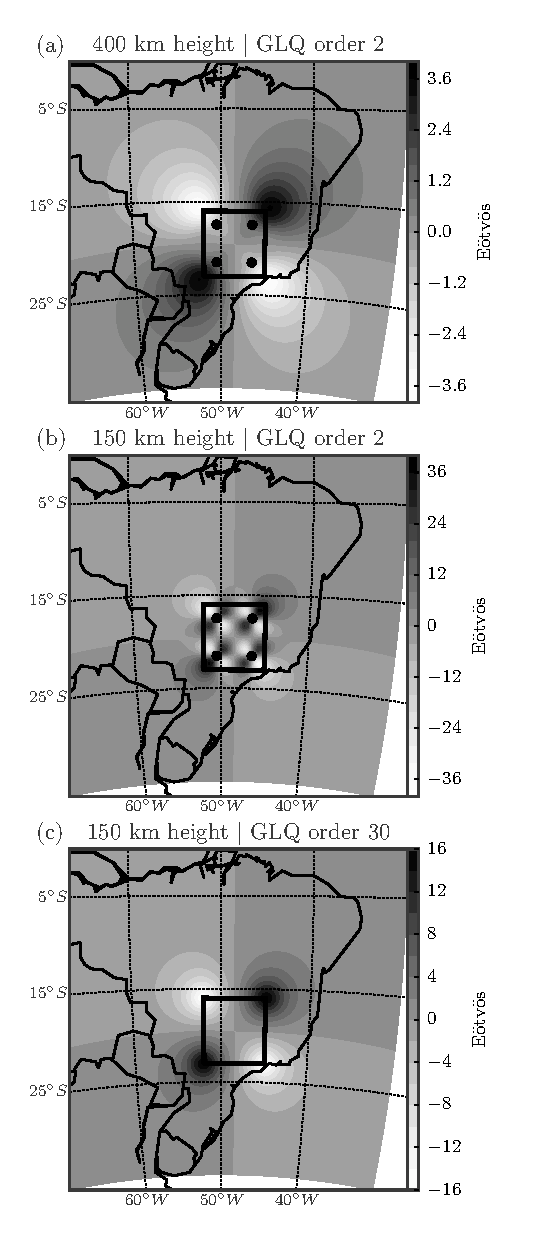
\includegraphics[width=0.5\textwidth]{figures/paper2/vary-height-and-order}
    \caption{
        Example of the effect of varying
        the computation height
        and the number of point masses in the Gauss-Legendre Quadrature.
        Black circles represent the horizontal location of the point masses.
        a) $g_{xy}$ calculated at $400\ km$ height using GLQ order 2
        ($2 \times 2 \times 2 = 8$ point masses).
        b) At $150\ km$ height and GLQ order 2,
        the result resembles that of
        four point masses instead of a single tesseroid.
        This effect was shown by \citet{ku1977}.
        c) At $150\ km$ but with a higher GLQ order of 30.
        In (c) the horizontal locations of the point masses were not shown.
        Notice that the results shown in (c) are similar to that expected
        for a single mass source.
    }
    \label{fig:p2-glqerrorsample}
\end{figure}


\subsection{Adaptive discretization}

\citet{li2011} proposed an alternative method
for decreasing the distance between point masses on the quadrature nodes
aiming at achieving an accurate integration.
Instead of increasing the GLQ order,
they keep it fixed to a given number
and divide the tesseroid into smaller volumes.
The sum of the effects of the smaller tesseroids
is equal to the gravitational effect of the larger tesseroid.
This division effectively decreases
the distance between nodes because
of the smaller size of the tesseroids.
The criterion for dividing a tesseroid is that the distance to the computation point
should be smaller than a constant times the size of the tesseroid.
This is analogous to the criterion proposed by \citet{ku1977}
because the size of the tesseroid serves as a proxy
for the distance between point masses.
This procedure is repeated recursively
until all tesseroids are within the acceptable
ratio of distance and size or a minimum size is achieved.

The advantage of this adaptive discretization is
that the number of point masses is only increased
in parts of the tesseroid that are
closer to the computation point.
Notice that the alternative approach of
simply increasing the order of the GLQ
would increase the number of point masses
evenly throughout the whole tesseroid.


%%%%%%%%%%%%%%%%%%%%%%%%%%%%%%%%%%%%%%%%%%%%%%%%%%%%%%%%%%%%%%%%%%%%%%%%%%%%%%
\section{Implementation}

We have implemented the calculation of
the tesseroid gravitational fields
with adaptive discretization
in version 1.2 of the open-source package \emph{Tesseroids}.
It is freely available online\footnote{
http://tesseroids.leouieda.com}\footnote{
http://dx.doi.org/10.5281/zenodo.16033}
under the BSD 3-clause open-source license.
An archived version of the source code
is also available as part of this article.

\emph{Tesseroids} consists of command-line programs
written in the C programming language.
The package includes programs to calculate
the gravitational fields of tesseroids and
rectangular prisms (in both Cartesian and spherical coordinates).
All programs receive input through
command-line arguments and the standard input channel (``STDIN'')
and output the results through the standard output channel (``STDOUT'').
For example,
the command to generate a regular grid with $NLON \times NLAT$ points,
 calculate $g_z$ and $g_{zz}$ caused by
the tesseroids in a file ``MODELFILE'',
and save the results to a file called ``OUTPUT''
is:

\begin{verbatim}
tessgrd -rW/E/S/N -bNLON/NLAT -zHEIGHT | \
    tessgz MODELFILE | \
    tessgzz MODELFILE > OUTPUT
\end{verbatim}

The \emph{src} folder of the source code archive
contains the C files that build the command-line programs
(e.g., \emph{tessgz.c}).
The \emph{src/lib} folder contains
the source files that implement the numerical computations.
We will not describe here the implementation of the input/output parsing and
other miscellanea.
Instead, we will focus on the details of the Gauss-Legendre Quadrature
integration of equations~\ref{eq:p2-tesspot}-\ref{eq:p2-tesstensor}
and the adaptive discretization of tesseroids.



\subsection{Numerical integration}

The source file \emph{src/lib/glq.c}
contains the code necessary to perform
a Gauss-Legendre Quadrature integration.
The first step in the GLQ is to compute the
locations of the discretization points (i.e., the point masses).
These points are roots of Legendre polynomials.
Precomputed values are available for low order polynomials,
typically up to order five.
For flexibility and to compute higher order roots,
we use the multiple root-finder algorithm of
\citet{barrera-figueroa2006}.
The additional computational load is minimal
because the root-finder algorithm
must be run only once per program execution.
The root-finder is implemented in functions
\emph{glq\_nodes} and \emph{glq\_next\_root}.
The computed roots will be in the range $[-1, 1]$
and must be scaled to the integration limits
(the physical boundaries of the tesseroid)
using function \emph{glq\_set\_limits} (see equation~\ref{eq:p2-glq_scaling}).

The GLQ weights (equation~\ref{eq:p2-glq_weights})
are computed by function \emph{glq\_weights}.
Both the computed roots and weights are stored in a data structure
(a C \emph{struct}) called \emph{GLQ}.
Function \emph{glq\_new}
handles memory allocation,
calculates the roots and weights,
and returns the complete \emph{GLQ} structure.

The numerical integration of the tesseroid gravitational fields
is performed by the functions in module \emph{src/lib/grav\_tess.c}.
Functions \emph{tess\_pot}, \emph{tess\_gx}, \emph{tess\_gy}, and so on,
compute the gravitational fields of a single tesseroid
on a single computation point.
These functions require three \emph{GLQ} structures,
each containing the roots and weights
for GLQ integration in the three dimensions.
The roots must be scaled to the
integration limits
$[\lambda_1, \lambda_2], [\phi_1, \phi_2], [r_1, r_2]$
(see equations~\ref{eq:p2-tesspot}-\ref{eq:p2-tesstensor}).
The integration consists of three loops
that sum the weighted kernel functions
evaluated at each GLQ point mass (the scaled roots).

The biggest bottlenecks for the numerical integration are
the number of point masses used
and the evaluation of the trigonometric functions in
equations~\ref{eq:p2-tesspot}-\ref{eq:p2-tesstensor} inside the inner loops.
Better performance is achieved
by pre-computing the sine and cosine of latitudes
and moving some trigonometric function evaluations
to the outer loops.


\subsection{Implementation of adaptive discretization}

Our implementation of the adaptive discretization algorithm
differs in a few ways from the one proposed by \citet{li2011}.
In \citet{li2011},
a tesseroid will be divided when
the smallest distance between it and the computation point
is smaller than a constant times
the largest dimension of the tesseroid.
Instead of the smallest distance,
we use the easier to calculate
distance between
the computation point $(r, \lambda, \phi)$
and the geometric center of the tesseroid
$(r_t, \lambda_t, \phi_t)$

\begin{equation}
    d = \left[
        r^2 + r_t^2 - 2 r r_t \cos\psi_t
        \right]^{\frac{1}{2}} ,
    \label{eq:p2-distance}
\end{equation}
\begin{equation}
    \cos\psi_t =
        \sin\phi\sin\phi_t + \cos\phi\cos\phi_t\cos(\lambda - \lambda_t) .
\end{equation}

Our definition of the dimensions of the tesseroid
(the ``side lengths'' of \citet{li2011})
along longitude, latitude, and radius, respectively, are
(Figure~\ref{fig:p2-division}a)

\begin{equation}
    L_\lambda = r_2 \arccos(\sin^2\phi_t +
        \cos^2\phi_t\cos(\lambda_2 - \lambda_1)),
    \label{eq:p2-sizelon}
\end{equation}
\begin{equation}
    L_\phi = r_2 \arccos(\sin\phi_2\sin\phi_1 + \cos\phi_2\cos\phi_1),
\end{equation}
\begin{equation}
    L_r = r_2 - r_1.
    \label{eq:p2-sizer}
\end{equation}

\noindent
$L_\lambda$ and $L_\phi$ are arc-distances measured along the top surface of
the tesseroid (Figure~\ref{fig:p2-division}a).
Specifically, $L_\lambda$ is measured long the middle latitude of the
tesseroid ($\phi_t$).

To determine if a tesseroid must be divided,
we check if

\begin{equation}
    \frac{d}{L_i} \geq D,
    \label{eq:p2-condition}
\end{equation}

\noindent
for each $i \in (\lambda, \phi, r)$.
$D$ is a positive scalar
hereafter referred to as the ``distance-size ratio''.
If the inequality holds for all three dimensions,
the tesseroid is not divided.
Thus, the distance-size ratio determines
how close the computation point can be
before we must divide the tesseroid.
The value of $D$ is indirectly responsible for
the accuracy of the solution and the computation time.
We will explore the relationship with the accuracy in the following section.

Figure~\ref{fig:p2-division} shows examples of
the resulting tesseroid models after adaptive discretization.
Figure~\ref{fig:p2-division}a shows
the initial tesseroid and computation point P.
Figures~\ref{fig:p2-division}b-d are
the result of adaptive discretization using
different values of the distance-size ratio $D$,
respectively,
$D=1$, $D=2$, and $D=6$.
The number of tesseroids in the resulting discretization is, respectively,
4, 38, and 936.

\begin{figure}
    \centering
    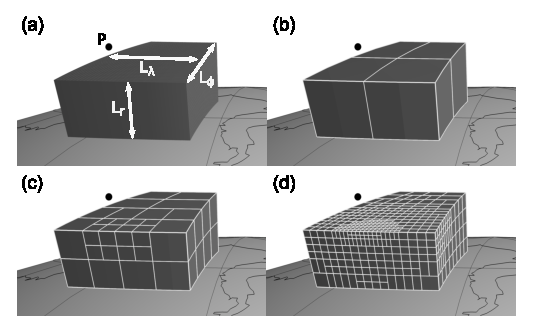
\includegraphics[width=\textwidth]{figures/paper2/tesseroid-split}
    \caption{
        Adaptive discretization
        of the tesseroid shown in (a)
        for a computation point P
        using the distance-size ratio $D$ equal to
        (b) 1, (c) 2, and (d) 6.
        $L_r$, $L_\phi$, and $L_\lambda$ are the dimensions of the tesseroid.
        Note that increasing $D$
        results in a fine division of the tesseroid
        close the computation point
        and a coarser division further away.
    }
    \label{fig:p2-division}
\end{figure}

Instead of using recursive function calls,
as originally proposed by \citet{li2011},
we use a stack-based implementation of the algorithm.
Stacks are array-like data structures
with a particular way of inserting and removing elements from it.
In a stack,
one can only insert elements to the top of the stack
(the last empty position).
Likewise,
one can only remove the last element of the stack
(commonly referred to as ``popping'' the stack).
Because of these restrictions,
stacks are also known as ``Last-In-First-Out'' (LIFO) data structures.

The discretization algorithm is implemented in
function \emph{calc\_tess\_model\_adapt}
of the file \emph{src/lib/grav\_tess.c}.
This function calculates the effect of a single tesseroid
on a single computation point.
The stack of tesseroids is represented by
the \emph{stack} variable,
an array of \emph{TESSEROID} structures.
We must define a maximum size for the stack to allocate memory for it.
Defining a maximum size allows us to
avoid an infinite loop
in case the computation point is on
(or sufficiently close to) the surface of the tesseroid.
We use the integer \emph{stktop}
to keep track of the index of
the last element in the stack (the top of the stack).

Below, we describe the algorithm to calculate
the effect of a single tesseroid from the input model
on a single computation point.
The algorithm starts by creating an empty stack of tesseroids.
Then, the stack is initialized with the single input tesseroid.
The initialization is done by copying the tesseroid into the stack
and setting \emph{stktop} to zero (the first element).
It is important to note that the stack is not the input tesseroid model.
Instead, it is a buffer used to temporarily store
each stage of the discretization algorithm.

Once the stack is initialized, the steps of the algorithm are:

\begin{enumerate}
    \item ``Pop'' the stack (i.e., take the last tesseroid from it).
        This will cause \emph{stktop} to be reduced by one.
        This tesseroid is the one that will be evaluated in the following
        steps.
    \item Compute the distance $d$ (equation~\ref{eq:p2-distance}) between
        the geometric center of the tesseroid and
        the computation point.
    \item Compute the dimensions of the tesseroid $L_\lambda$, $L_\phi$,
        and $L_r$ using equations~\ref{eq:p2-sizelon}-\ref{eq:p2-sizer}.
    \item Check the condition in equation~\ref{eq:p2-condition} for each
        dimension of the tesseroid.
    \item If all dimensions hold the inequality \ref{eq:p2-condition},
        the tesseroid is not divided and its
        gravitational effect is computed using the
        Gauss-Legendre Quadrature
        (equations~\ref{eq:p2-tesspot}-\ref{eq:p2-tesstensor} and~\ref{eq:p2-glq3d}).
        We use a GLQ order of two for all three dimensions
        ($2 \times 2 \times 2 = 8$ point masses)
        by default.
        This value can be changed using
        a command-line argument of the modeling programs.
    \item If any of the dimensions fail the condition:
    \begin{enumerate}
        \item Divide the tesseroid in half along each dimension that failed
             the condition.
        \item Check if there is room in the stack
            for the new tesseroids
            (i.e.,the number of new elements plus \emph{stktop}
             is smaller than the maximum stack size).
             If there isn't,
             warn the user of a ``stack overflow''
             and compute the effect of the tesseroid, as in step 5.
             If there is room in the stack,
             place the smaller tesseroids into
             the stack.
    \end{enumerate}
    \item Repeat the above steps until the stack is empty
        (\emph{stktop} is equal to -1).
\end{enumerate}

The algorithm above is repeated
for every tesseroid of the input model
and the results are summed.
This will yield the gravitational effect
of the input tesseroid model on a single point.
Thus, the computations must be repeated
for every computation point.
The whole algorithm can be summarized
in the following pseudo-code.

\begin{verbatim}
Initialize the output array with zeros.
for tesseroid in model:
  for point in grid:
    Initialize the stack with tesseroid.
    stktop = 0
    while stktop >= 0:
      Perform steps 1-6 of the algorithm.
    Sum the calculated value to the output.
\end{verbatim}

This stack-based implementation
has some advantages over the original recursive implementation,
namely:
(1) It gives the developer more control over the recursion step.
(2) In general, it is faster because it bypasses the overhead of function
calls.
In recursive implementations,
the developer has no control over
the maximum number of consecutive recursive calls
(i.e., the ``recursion depth'').
This limit may vary with programming language,
compiler, and operating system.
Overflowing the maximum recursion depth
may result in program crashes,
typically with cryptic or inexistent error messages.
In the stack-based implementation,
the developer has complete control.
Overflowing of the stack can be handled gracefully
with an error message
or even performing a suitable approximation of the result.

\subsection{Code for figures and error analysis}


The error analysis and all figures in this article
were produced in IPython notebooks
\citep{perez2007}.
The notebook files combine source code in various programming languages,
program execution,
text, equations,
and the figures generated by the code
into a single document.
We used the following Python language libraries
to perform the error analysis and generate figures:
\emph{pandas} by \citet{mckinney2010},
\emph{matplotlib} by \citet{hunter2007} for 2D figures and maps,
and \emph{Mayavi} by \citet{ramachandran2011} for 3D figures.

The IPython notebooks
and the data generated for the error analysis,
as well as instructions for installing the software
and running the programs,
are also included in
the source code archive that accompanies this article.
Alternatively,
all accompanying material is available
in an online repository\footnote{
https://github.com/pinga-lab/paper-tesseroids}.



%%%%%%%%%%%%%%%%%%%%%%%%%%%%%%%%%%%%%%%%%%%%%%%%%%%%%%%%%%%%%%%%%%%%%%%%%%%%%%
\section{Evaluation of the accuracy}



The key controlling point of the adaptive discretization algorithm
is the distance-size ratio $D$ (equation~\ref{eq:p2-condition}).
The specific value chosen for $D$ determines how many divisions will be made
(Figure~\ref{fig:p2-division}).
Thus, $D$ indirectly controls both the accuracy of the integration
and the computation time.
In this section, we investigate the relationship between
the distance-size ratio and the integration error.
We perform the analysis for the gravitational potential,
acceleration, and gradient tensor components
to evaluate if the same value of $D$ yields compatible error levels
for different fields.

The reference against which we compare the computed tesseroid fields
is a homogeneous spherical shell.
The shell has analytical solutions along the polar axis
\citep{lafehr1991a, mikuska2006, grombein2013}
and can be perfectly discretized into tesseroids.
We chose a spherical shell with a thickness of 1 km,
density of $2670\ kg.m^{-3}$,
bottom at height 0 km above the reference sphere,
and top at 1 km height.
We produced tesseroid models of the shell by discretizing it along the
horizontal dimensions into a regular mesh.


Figure~\ref{fig:p2-glqerrorsample} shows that the largest errors are spread over
on top of the tesseroid.
Thus, calculating the tesseroid fields at a single point might not
capture the point of largest error.
Instead, we calculate the effect of the tesseroid model on a regular grid
of $10 \times 10$ points at different geographic locations
(see Table~\ref{tbl:experiment}).
Fortunately, the symmetry of the shell allows us to consider the computation
point at any geocentric coordinate.
Therefore, the effect of the shell will be same along the entire grid.
We compute the differences between the effects of the shell and the tesseroid
model on the grid.
However, we will consider only the largest error in our analysis.


We placed the grid on top of a particular tesseroid
to increase the chances of capturing the true largest integration error.
We calculate the errors for values of the distance-size ratio
$D$ varying from 0 (i.e., no divisions) to 10 in 0.5 intervals.
Furthermore, we repeated the error analysis in four different numerical experiments,
each with computation grids at different locations and
different tesseroid model sizes.
Table~\ref{tbl:experiment} describes the different numerical
experiments and the corresponding parameters of the computation grid and
tesseroid model.


Figure~\ref{fig:p2-dist-size-curves} shows
the maximum difference between the shell and tesseroid fields
as a function of $D$ for the four experiments.
The differences are given as a percentage of the shell value.
We established a maximum tolerated error of $0.1\%$, represented by the
horizontal solid lines in Figure~\ref{fig:p2-dist-size-curves}.
Only results for the gravitational potential, $g_z$, and $g_{zz}$ are shown.
The results for the other diagonal components of the gravity gradient tensor
are similar to $g_{zz}$.
Figures for these components can be found in the supplementary material
(see section "Reproducing the analysis and results").


For the potential $V$, a distance-size ratio $D=1$ guarantees that the curves
for all experiments are below the $0.1\%$ error threshold.
For $g_z$, the same is achieved with $D=1.5$.
Conversely, $g_{zz}$ requires a value of $D=8$ to achieve an error level of
$0.1\%$.
For a computation height of 260 km, the error curve for $g_{zz}$
intercepts the error threshold line at $D=2.5$.
This behavior suggests that the error curves for $g_{zz}$ might depend on the
computation height.
To test this hypothesis, we computed the error curves for $g_{zz}$ at
heights 2, 10, 50, 150, and 260 km.
Figure~\ref{fig:p2-gzz-with-height} shows the results for $g_{zz}$ at varying
computation heights.
Notice that the distance-size ratio required to achieve $0.1\%$ accuracy
decreases as the computation height increases.
For example, computation at 260 km height requires $D=2.5$ whereas at 10 km
height a value of $D=5.5$ is required to achieve the same accuracy.
One can take advantage of this behavior to reduce the distance-size ratio for
computations of the gravity gradient tensor at high altitudes,
saving computation time.


We have implemented the values of the distance-size ratio producing $0.1\%$
accuracy determined above as defaults for the software \emph{Tesseroids}.
We chose the conservative value of $D=8$ for the gravity gradient components
as a fail-safe alternative.
Users can control the value of $D$ used in the computations through
command-line arguments to achieve greater performance at the cost of
accuracy.


\begin{table*}
\centering
\begin{tabular}{lccc}
    \hline
    ~             & Grid location & Grid height & Tesseroid size \\
    \hline
    Experiment 1 (pole)            & 89N--90N/0E--1E  & 2 km   & $1^\circ \times 1^\circ$ \\
    Experiment 2 (equator)         & 0N--1N/0E--1E    & 2 km   & $1^\circ \times 1^\circ$ \\
    Experiment 3 (260 km)          & 89N--90N/0E--1E  & 260 km & $1^\circ \times 1^\circ$ \\
    Experiment 4 ($30^\circ$ size) & 60N--90N/0E--30E & 2 km   & $30^\circ \times 30^\circ$ \\
    \hline
\end{tabular}
\caption{
    Parameters of the numerical experiments to quantify the accuracy of
    the numerical integration.
    All grids had $10\times10$ regularly spaced computation points at a
    constant height.
    Tesseroids used to discretize the spherical shell had 1 km thickness and
    the horizontal dimensions shown in the table.
}
\label{tbl:experiment}
\end{table*}

\begin{figure}
    \centering
    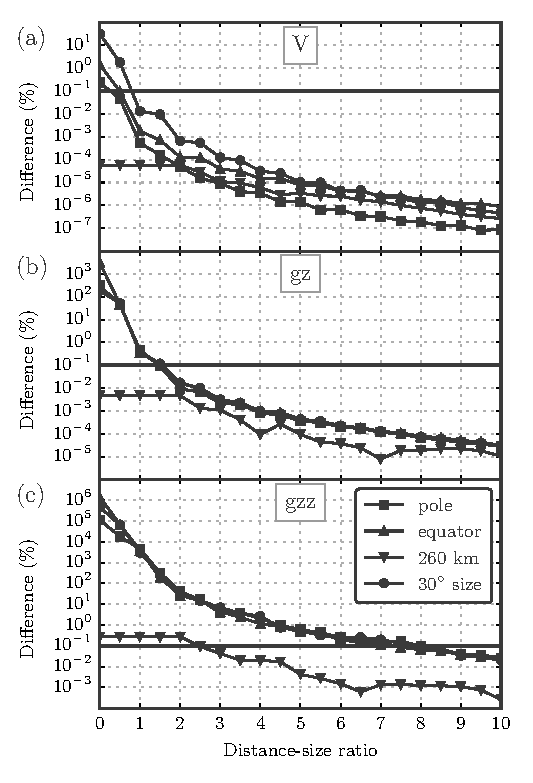
\includegraphics{figures/paper2/distance-size-curves}
    \caption{
        The maximum difference between the computed tesseroid and shell effects
        as a function of the distance-size ratio $D$
        for (a) the gravitational potential, (b) $g_z$, and (c) $g_{zz}$.
        The difference is given as a percentage of the shell effect.
        Curves correspond to the different tesseroid models and computation
        grids shown in Table~\ref{tbl:experiment}.
        The horizontal solid black line marks the established error threshold
        of $0.1\%$.
        A value of $D=0$ means that no divisions are made.
    }
    \label{fig:p2-dist-size-curves}
\end{figure}

\begin{figure}
    \centering
    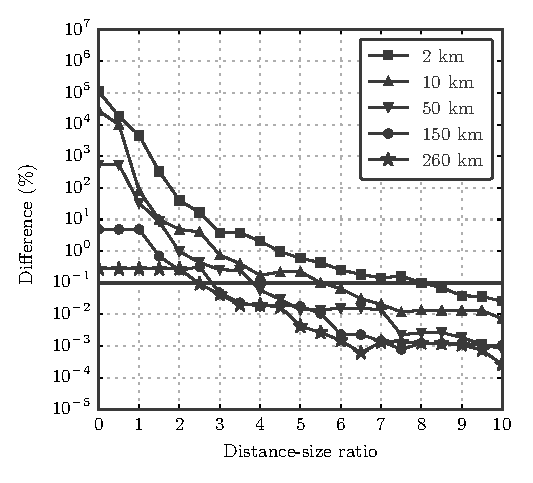
\includegraphics{figures/paper2/gzz-with-height}
    \caption{
        Difference between the computed $g_{zz}$ for the spherical shell and
        the tesseroid model at different heights. Curves show the maximum
        difference as a percentage of the shell value.
        The horizontal solid black line marks the established error threshold
        of $0.1\%$.
        A value of $D=0$ means that no divisions are made.
    }
    \label{fig:p2-gzz-with-height}
\end{figure}


%%%%%%%%%%%%%%%%%%%%%%%%%%%%%%%%%%%%%%%%%%%%%%%%%%%%%%%%%%%%%%%%%%%%%%%%%%%%%%
\section{Conclusions}


We have presented the open-source software \emph{Tesseroids}.
It consists of command-line programs,
written in the C programming language,
to perform the forward modeling of gravitational fields in spherical
coordinates.
The fields are calculated from a mass model composed of spherical prisms, the
so-called tesseroids.
The volume integrals of the gravitational fields of a tesseroid are solved
numerically using the Gauss-Legendre Quadrature (GLQ).
The GLQ approximates the volume integrals by weighted sums of point mass
effects.
The error of the GLQ integration increases as the computation point gets closer
to the tesseroid.
To counter this effect,
the accuracy of the GLQ integration can be increased by using more point
masses or by dividing each tesseroid into smaller ones.


We have implemented and improved upon an adaptive discretization algorithm to
achieve an optimal division of tesseroids.
Tesseroids are divided into more parts closer to the computation point,
where more point masses are needed.
Our implementation of the adaptive discretization uses a ``stack'' data
structure in place of the originally proposed recursive implementation.
As a rule of thumb in procedural languages (like C),
stack-base implementations are computationally faster
than the equivalent code using function recursion.
Furthermore, the stack-based algorithm allows more control
over errors when too many divisions are necessary.
The adaptive discretization is controlled by
a scalar called the distance-size ratio ($D$).
The algorithm ensures that all tesseroids will
have dimensions smaller than $D$ times the distance to the computation point.
The value of $D$ indirectly controls the accuracy of the integration as well as
the computation time.


We performed an error analysis to determine
the optimal value of $D$ required to achieve a target accuracy.
We used a spherical shell as a reference to calculate the computation error of
our algorithm for different values of $D$.
Our results show that the values of $D$ required to achieve a maximum error
of 0.1\% of the shell values are
1 for the gravitational potential, 1.5 for the gravitational acceleration,
and 8 for the gravity gradients.
Previous assumptions in the literature
were that accurate results are guaranteed if
the distance to the tesseroid is larger than
the distance between point masses.
This condition was previously applied indiscriminately
to both the gravitational acceleration and the gravity gradients.
That assumption is equivalent to using $D=1.5$ for all fields.
Our results show that this is valid for the gravitational
acceleration and results in a 0.1\% computation error.
This is expected because the original study that determined the above condition
was performed on the vertical component of gravitational acceleration.
However, applying the same condition to the gravity gradients produces
an error of the order of $10^2\%$.


For the gravity gradients in particular,
the distance-size ratio required for 0.1\% error decreases with height.
We believe this is because the decay factor for
the gravity gradient components is $d^{-3}$,
whereas the discretization algorithm uses $d/L_i$.
As the computation point becomes closer to the tesseroid,
the field increases more rapidly than
the algorithm increases the amount of discretization.
Hence, a higher value of D (i.e., more discretization)
is required.


The values of the distance-size ratio determined above were
incorporated as defaults in the software \emph{Tesseroids}.
We chose the value $D=8$ for the gravity gradients as a conservative default.
If the user desires, the value of $D$ used can be controlled by a command-line
argument.


In situations that require many tesseroid divisions,
the stack used in the algorithm will overflow and further
divisions become impossible.
The current implementation warns the user that
the overflow occurred and proceeds with the GLQ integration without division.
Future improvements to the algorithm include a better way to handle such
situations as they arise.
An alternative would be to replace the tesseroid by an equivalent
right rectangular prism and compute its effects instead.
This would allow accurate computations at smaller distances.
Furthermore,
the computation time increases drastically as the computation point
gets closer to the tesseroid.
This effect can be prohibitive for computing the gravity gradients at
relatively low heights (e.g., for terrain corrections of
ground or airborne surveys).
Further investigation of different criteria for dividing the tesseroids could
yield better performance through a reduced number of divisions.


%%%%%%%%%%%%%%%%%%%%%%%%%%%%%%%%%%%%%%%%%%%%%%%%%%%%%%%%%%%%%%%%%%%%%%%%%%%%%%
\section{Acknowledgments}

The authors were supported in this research by
a fellowship (VCFB) from
Conselho Nacional de Desenvolvimento Cient\'ifico e Tecnol\'ogico (CNPq)
and a scholarship (LU) from
Coordena\c{c}\~ao de Aperfei\c{c}oamento de Pessoal de N\'ivel Superior
(CAPES),
Brazil.
Additional support for the authors was provided by
the Brazilian agency FAPERJ (grant E-26/103.175/2011)
and by the GOCE-Italy project (ASI).

\chapter{Fast non-linear gravity inversion in spherical coordinates with
         application to the South American Moho}


This chapter has been submitted for publication in the Geophysical Journal
International.

\section{Abstract}

Estimating the relief of the Moho from gravity data is a computationally
intensive non-linear inverse problem.
What is more, the modeling must take the Earths curvature into account when
the study area is of regional scale or greater.
We present a regularized non-linear gravity inversion method that has a low
computational footprint and employs a spherical Earth approximation.
To achieve this, we combine the highly efficient Bott's method with
smoothness regularization and a discretization of the anomalous Moho into
tesseroids (spherical prisms).
The computational efficiency of our method is attained by harnessing the
fact that all matrices involved are sparse.
The inversion results are controlled by three hyper-parameters: the
regularization parameter, the anomalous Moho density-contrast, and the
reference Moho depth.
We estimate the regularization parameter using the method of hold-out
cross-validation.
Additionally, we estimate the density-contrast and the reference depth
using knowledge of the Moho depth at certain points.
We apply the proposed method to estimate the Moho depth for the South
American continent using satellite gravity data and seismological data.
The final Moho model is in accordance with previous gravity-derived models
and seismological data.
The misfit to the gravity and seismological data is worse in the Andes and
best in oceanic areas, central Brazil and Patagonia, and along the Atlantic
coast.
Similarly to previous results, the model suggests a thinner crust of 30-35
km under the Andean foreland basins.
Discrepancies with the seismological data are greatest in the Guiana
shield, the central Solimões and Amazon basins, the Paraná basin, and the
Borborema province.
These differences suggest the existence of crustal or mantle density
anomalies that were unaccounted for during gravity data processing.


%%%%%%%%%%%%%%%%%%%%%%%%%%%%%%%%%%%%%%%%%%%%%%%%%%%%%%%%%%%%%%%%%%%%%%%%%%%%%%%
\section{Introduction}

The Mohorovičić discontinuity (or Moho) that marks the transition from the
crust to the mantle, is studied almost exclusively through indirect geophysical
methods.
The two main methods used to estimate the depth of the Moho are seismology,
with both natural and controlled sources, and gravimetry.
With the advent of satellite gravimetry missions like GRACE and GOCE,
gravity derived crustal models can be produced in regional or global scales
\citep[e.g. ][]{reguzzoni2013,vandermeijde2013,vandermeijde2015}.
New spherical harmonic gravity models that use these satellite observation,
like GOCO5S \citep{mayer-guerr2015}, provide almost homogeneous data coverage
in difficult to access regions traditionally poor in terrestrial data.
An example is South America, where seismologic and terrestrial gravity data
are traditionally concentrated around large urban centers and coastal areas.

Estimating Moho depth from gravity data is a non-linear inverse problem.
One can generalize this problem to estimating the relief of an interface,
such as the basement of a sedimentary basin or the relief of the anomalous
Moho.
Several methods have been developed over the years to solve this inverse
problem, for example
\citet{bott1960, barbosa1999b, barbosa1999a, barnes2012, leao1996, martins2010,
martins2011, oldenburg1974, reguzzoni2013, santos2015, silva2006, silva2014},
to name a few.
Solving the inverse problem is computationally demanding because it requires
the construction of large dense matrices and the solution of large linear
systems.
As a result, some authors search for ways to increase the computational
efficiency of this class of inverse problem.
\citet{bott1960} proposed a method based on iteratively applying corrections to
a starting estimate based on the inversion residuals.
The algorithm is fast because it bypasses the construction and solution of
linear systems and only involves forward modeling.
\citet{oldenburg1974} showed that the fast FFT-based forward modeling of
\citet{parker1973} could be rearranged to estimate the relief.
\citet{barnes2012} use a form of adaptive discretization to compute the
Jacobian, or sensitivity, matrix.
For each data point, the discretization will be progressively coarser
the further way from the point.
This reduces the matrix and, consequently, the linear systems to a sparse form
that can be solved efficiently.
Recently, \citet{silva2014} extended and generalized the original method of
\citet{bott1960} and \citet{santos2015} used this extension to estimate a
basement relief with sharp boundaries.

Most non-linear gravity inversion methods discretize the relief of the
interface into juxtaposed right-rectangular prisms with a known density
contrast.
The inverse problem is then to estimate the thickness of each prism from the
gravity data.
The use of rectangular prisms implies a planar Earth approximation and may not
be adequate for continental and global scale studies.
In such cases, a spherical Earth approximation is preferred.
\citet{wieczorek1998} developed a spherical harmonic equivalent of the
Parker-Oldenburg FFT algorithm and applied it to estimate the crustal structure
of the Moon.
\citet{reguzzoni2013} use a spherical approximation to estimate the global
Moho relief from GOCE satellite gravity data.
Conversely, one could adapt one of the methods developed for
right-rectangular prisms to use tesseroids (spherical prisms) instead.
One of the difficulties of this approach is that the forward problem for a
tesseroid must be solved numerically.
Two alternatives proposed in the literature to the numerical solution are
Taylor series expansion \citep{heck2007, grombein2013}
and the Gauss-Legendre Quadrature
\citep{asgharzadeh2007}.
Numerical experiments by \citet{wild-pfeiffer2008} suggest that the
Gauss-Legendre Quadrature (GLQ) offers superior results.
However, the GLQ suffers from numerical instability when the computation point
is close to the tesseroid \citep{asgharzadeh2007}.
To overcome the numerical instability, \citet{li2011} proposed an adaptive
discretization algorithm which was later improved upon by \citet{uieda2016}.

In any gravity inversion for the relief of an interface, two hyper-parameters
control the inversion results: the density-contrast between the two mediums
and the reference level around which the interface undulates.
The reference level is the depth of the Normal Earth Moho in the case of the
anomalous Moho.
For regularized inversions, an additional hyper-parameter is the regularization
parameter that balances data-misfit and regularization.
The two most commonly used methods for estimating the regularization parameter
are the L-curve criterion and Generalized Cross Validation (GCV).
\citet{farquharson2004} provide for a thorough comparison of both methods.
Estimating the density-contrast in a sedimentary basin context has been tackled
by \citet{silva2006} and \citet{martins2010} when the basement depth is known
at a few points.
To the authors knowledge no attempt has been made to estimate the reference
level.

We present a non-linear gravity inversion to estimate the Moho depth in
a spherical Earth approximation.
Our method is based on the \citet{silva2014} Gauss-Newton formulation of the
method of \citet{bott1960}.
We use tesseroids to discretize the anomalous Moho and the adaptive
discretization algorithm of \citet{uieda2016} for the forward modeling.
The stability of the inversion is achieved through smoothness regularization.
In order to maintain the computational efficiency of Bott's method,
we exploit the sparse nature of all matrices involved in the computations.
We employ a variant of GCV known as hold-out cross-validation \citep{kim2009}
to estimate the regularization parameter.
Additionally, we estimate the density-contrast and reference level
simultaneously in a second cross-validation.
Similarly to \citet{silva2006} and \citet{martins2010}, this cross-validation
procedure uses knowledge of the Moho depth at certain points.
Finally, we apply the proposed method to estimate the Moho depth for South
America using gravity data from the GOCO5S model \citep{mayer-guerr2015} and
the seismological data of \citet{assumpcao2013a}.



%%%%%%%%%%%%%%%%%%%%%%%%%%%%%%%%%%%%%%%%%%%%%%%%%%%%%%%%%%%%%%%%%%%%%%%%%%%%%%%
\section{Methodology}

In potential field methods,
we must isolate the target anomalous density distribution prior to modeling and
inversion.
In our case, the target is the relief of the real Moho undulating around a
reference Moho.
We do this by removing all other effects from the gravity observations.
The first correction is to remove the
scalar gravity of an ellipsoidal reference Earth (the Normal Earth),
hereafter denoted as $\gamma$.
This effect is calculated on the same point $P$ where
the gravity observation was made
(Fig~\ref{fig:p3-anomalysketch}a-b).
$\gamma(P)$ is calculated using
the closed-form solution presented by \citet{li2001a}.
The difference between the observed gravity at point P ($g(P)$)
and Normal gravity at the same point
is known as the gravity disturbance,

\begin{equation}
    \delta(P) = g(P) - \gamma(P).
    \label{eq:p3-disturbance}
\end{equation}

The disturbance contains only the gravitational effects of density
distributions that are anomalous with respect to the Normal Earth
(see Fig.~\ref{fig:p3-anomalysketch}c).
This includes all masses above the surface of the ellipsoid (the topography),
the mass deficiency of the oceans,
the mass deficiency of sedimentary basins,
crustal sources (e.g., igneous intrusions, lateral density changes, etc),
heterogeneities below the upper mantle,
and the effect of the difference between the real Moho
topography and the Moho of the Normal Earth.

In order to invert for the anomalous Moho relief,
we must first isolate its gravitational attraction.
Thus, all other effects
must be either removed or assumed negligible.
Here, we will remove the effect of the topography and oceans
in order to obtain the full Bouguer disturbance
(Fig~\ref{fig:p3-anomalysketch}d),

\begin{equation}
    \delta_{bg}(P) = \delta(P) - g_{topo}(P).
    \label{eq:p3-bouguer}
\end{equation}

\noindent
We will remove the effect of sedimentary basins
but assume that the effects of
other crustal and mantle sources are negligible.
Thus, the only effect left will be that of the anomalous Moho relief
(Fig~\ref{fig:p3-anomalysketch}e).
The gravitational attraction of the topography, oceans, and basins are
calculated in a spherical Earth approximation by forward modeling using
tesseroids (Fig.~\ref{fig:p3-tesseroid}).
The tesseroid effects are calculated numerically using
Gauss-Legendre Quadrature (GLQ) integration \citep{asgharzadeh2007}.
The accuracy of the GLQ integration is improved by the adaptive discretization
scheme of \citet{uieda2016}.


\begin{figure}
    \centering
    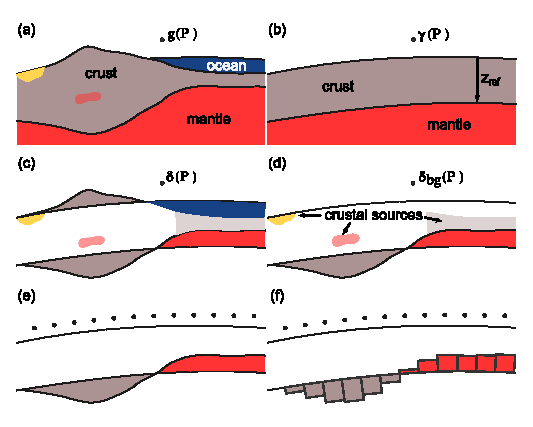
\includegraphics[width=0.7\textwidth]{figures/paper3/problem-concept}
    \caption{
        Sketch of the stages in gravity data correction and
        the discretization of the anomalous Moho relief using tesseroids.
        (a) The Earth and the measured gravity at point P ($g(P)$).
        (b) The Normal Earth and the calculated normal gravity at point P
        ($\gamma(P)$). $z_{ref}$ is the depth of the Normal Earth Moho.
        (c) The gravity disturbance ($\delta(P)$) and
        the corresponding density anomalies after removal of the normal gravity:
        topography, oceans, crustal heterogeneities, and the anomalous Moho.
        (d) The Bouguer disturbance ($\delta_{bg}(P)$) after topographic
        correction and the remaining density anomalies.
        (e) All density anomalies save the anomalous Moho are assumed to have
        been removed before inversion.
        (f) The discretization of the anomalous Moho in tesseroids. Grey
        tesseroids will have a negative density contrast while red tesseroids
        will have a positive one.
    }
    \label{fig:p3-anomalysketch}
\end{figure}

\begin{figure}
    \centering
    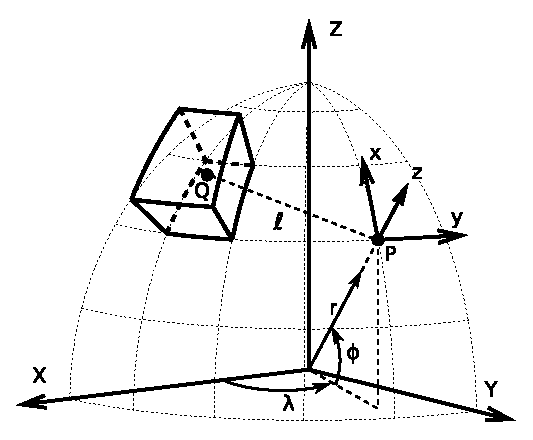
\includegraphics{figures/paper3/tesseroid-coord-sys}
    \caption{Sketch of a tesseroid (spherical prism) in a geocentric coordinate
        system (X, Y, Z).
        Observations are made at point P with respect to it's local
        North-oriented coordinate system (x, y, z).
        After \citet{uieda2015}.
    }
    \label{fig:p3-tesseroid}
\end{figure}


%%%%%%%%%%%%%%%%%%%%%%%%%%%%%%%%%%%%%%%%%%%%%%%%%%%%%%%%%%%%%%%%%%%%%%%%%%%%%%%
\subsection{Parametrization}

We parameterize the forward problem by discretizing the anomalous Moho
into a grid of $M_{lon} \times M_{lat} = M$ juxtaposed tesseroids
(Fig~\ref{fig:p3-anomalysketch}f).
The true (real Earth) Moho varies in depth
with respect to the Moho of the Normal Earth.
Hereafter we will refer to the depth of the Normal Earth Moho as $z_{ref}$
(see Fig.~\ref{fig:p3-anomalysketch}b).
In cases where the true Moho is above $z_{ref}$,
the top of the $k$th tesseroid is the Moho depth $z_{k}$,
the bottom is $z_{ref}$, and the density-contrast ($\Delta\rho$) is positive
(red tesseroids in Fig~\ref{fig:p3-anomalysketch}f).
If the Moho is below $z_{ref}$, the top of the tesseroid is $z_{ref}$,
the bottom is $z_k$, and $\Delta\rho$ is negative
(grey tesseroids in Fig~\ref{fig:p3-anomalysketch}f).

Considering that the absolute value of the density-contrasts
of the tesseroids is a fixed parameter,
the predicted gravity anomaly of the Moho is a non-linear function of the
parameters $z_k$, $k=1, \ldots, M$,

\begin{equation}
    d_i = f_i(\mathbf{p}),
    \label{eq:p3-forward}
\end{equation}

\noindent in which $d_i$ is the $i$th element of the $N$-dimensional predicted
data vector $\mathbf{d}$, $\mathbf{p}$ is the $M$-dimensional parameter vector
containing the $M$ Moho depths ($z_k$),
and $f_i$ is the $i$th non-linear function that maps the parameters onto the
data.
The functions $f_i$ are the radial component of the gravitational attraction
of the tesseroid Moho model.



%%%%%%%%%%%%%%%%%%%%%%%%%%%%%%%%%%%%%%%%%%%%%%%%%%%%%%%%%%%%%%%%%%%%%%%%%%%%%%%
\subsection{Inverse problem}

We wish to estimate the parameter vector $\mathbf{p}$ from a set of observed
gravity anomaly data $\mathbf{d}^o$.
The least-squares estimate is the one that minimizes the data-misfit function

\begin{equation}
    \phi(\mathbf{p}) =
    [\mathbf{d}^o - \mathbf{d}(\mathbf{p})]^T[\mathbf{d}^o - \mathbf{d}(\mathbf{p})].
    \label{eq:p3-data-misfit}
\end{equation}

Function $\phi(\mathbf{p})$ is non-linear with respect to $\mathbf{p}$.
Thus, we can determine its minimum using gradient-based
iterative optimization
methods like Gauss-Newton or Steepest Descent.
Such methods start from an initial estimate $\mathbf{p}^0$ and iteratively
update the estimate until a minimum is reached.

For the Gauss-Newton method,
the update at the $k$th iteration,
$\mathbf{\Delta p} = \mathbf{p}^{k+1} - \mathbf{p}^k$,
is the solution of the linear system

\begin{equation}
    \mathbf{H}^k\mathbf{\Delta p} = -\mathbf{\nabla\phi}^k,
    \label{eq:p3-gaussnewton}
\end{equation}

\noindent in which
$\mathbf{\nabla\phi}^k$ and $\mathbf{H}^k$ are, respectively,
the gradient vector and the Hessian matrix of $\phi(\mathbf{p})$.

The Steepest Descent method uses only the gradient direction
to update the initial estimate \citep{kelley1987}.
The update at the $k$th iteration is achieved by equating the Hessian
in Eq.~\ref{eq:p3-gaussnewton} to the identity matrix,

\begin{equation}
    \mathbf{\Delta p} = -\mathbf{\nabla\phi}^k.
    \label{eq:p3-steepest}
\end{equation}

\noindent
Thus, it does not require the computation and storage of the Hessian matrix
nor the solution of linear systems.
However, the Steepest Descent method has poor convergence when the
current solution is close to the minimum of the goal function
\citep{kelley1987}.

The gradient vector and the Gauss-Newton approximation of the Hessian matrix
of $\phi(\mathbf{p})$ are, respectively,

\begin{equation}
    \mathbf{\nabla\phi}^k = -2\mathbf{A}^T[\mathbf{d}^o - \mathbf{d}(\mathbf{p}^k)],
    \label{eq:p3-gradient}
\end{equation}

\noindent
and

\begin{equation}
    \mathbf{H}^k \approx 2\mathbf{A}^T\mathbf{A},
    \label{eq:p3-hessian}
\end{equation}

\noindent in which
$\mathbf{A}$ is the Jacobian or sensitivity matrix,

\begin{equation}
    A_{ij} = \dfrac{\partial f_i}{\partial p_j}(\mathbf{p^k}).
    \label{eq:p3-jacobian}
\end{equation}



%%%%%%%%%%%%%%%%%%%%%%%%%%%%%%%%%%%%%%%%%%%%%%%%%%%%%%%%%%%%%%%%%%%%%%%%%%%%%%%
\subsection{Regularization}

Non-linear inversions for the relief of an interface (like the Moho)
are ill-posed and require additional constraints in the form of
regularization \citep{silva2001}.
A common approach is to use the first-order Tikhonov regularization to impose
smoothness on the solution.
The cost function for smoothness regularization is given by

\begin{equation}
    \theta(\mathbf{p}) = \mathbf{p}^T\mathbf{R}^T\mathbf{R}\mathbf{p},
    \label{eq:p3-regul}
\end{equation}

\noindent where $\mathbf{R}$ is an $L \times M$ finite-difference matrix
representing the $L$ first-order differences between adjacent tesseroids.

The solution $\hat{\mathbf{p}}$ to the regularized inverse problem is the one that
minimizes the goal function

\begin{equation}
    \Gamma(\mathbf{p}) = \phi(\mathbf{p}) + \mu\theta(\mathbf{p}),
    \label{eq:p3-goalfunction}
\end{equation}

\noindent
in which $\mu$ is the regularization parameter that controls the balance
between fitting the observed data and obeying the smoothness constraint.

The goal function $\Gamma(\mathbf{p})$ is also non-linear with respect to
$\mathbf{p}$ and can be minimized using the Gauss-Newton or Steepest Descent
methods.
The gradient vector and Hessian matrix of the goal function are, respectively,

\begin{equation}
    \mathbf{\nabla\Gamma}^k =
        -2\mathbf{A}^T[\mathbf{d}^o - \mathbf{d}(\mathbf{p}^k)] +
        2\mu\mathbf{R}^T\mathbf{R}\mathbf{p}^k,
    \label{eq:p3-gradient-regul}
\end{equation}

\noindent and

\begin{equation}
    \mathbf{H}^k = 2\mathbf{A}^T\mathbf{A} + 2\mu\mathbf{R}^T\mathbf{R}.
    \label{eq:p3-hessian-regul}
\end{equation}

\noindent The parameter updates for the regularized Gauss-Newton and Steepest
Descent methods, respectively, then become

\begin{equation}
    \left[\mathbf{A}^T\mathbf{A} + \mu\mathbf{R}^T\mathbf{R}\right]
    \mathbf{\Delta p} =
        \mathbf{A}^T[\mathbf{d}^o - \mathbf{d}(\mathbf{p}^k)] -
        \mu\mathbf{R}^T\mathbf{R}\mathbf{p}^k,
    \label{eq:p3-gaussnewton-regul}
\end{equation}

\noindent and

\begin{equation}
    \mathbf{\Delta p} =
        \mathbf{A}^T[\mathbf{d}^o - \mathbf{d}(\mathbf{p}^k)] -
        \mu\mathbf{R}^T\mathbf{R}\mathbf{p}^k,
    \label{eq:p3-steepest-regul}
\end{equation}

Producing the regularized solution using the above equations is computationally
costly because of two main factors:
(1) the evaluation and storage of the dense $N \times M$ Jacobian matrix
$\mathbf{A}$
and (2) the solution of the resulting $M \times M$ equation system
(not required for Steepest Descent).
In practice, the derivatives in the Jacobian (Eq.~\ref{eq:p3-jacobian})
are often calculated through a first-order finite-difference approximation.
Thus, evaluating $\mathbf{A}$ requires $2\times M \times N$ forward modeling
operations for each iteration of the gradient descent algorithm.
These computations are performed for each iteration of the optimization.


%%%%%%%%%%%%%%%%%%%%%%%%%%%%%%%%%%%%%%%%%%%%%%%%%%%%%%%%%%%%%%%%%%%%%%%%%%%%%%%
\subsection{Bott's method}

\citet{bott1960} developed an efficient method to determined the basement
relief of a sedimentary basin from gravity observations.
The method requires data on a regular grid of $N_x \times N_y = N$
observations.
The basement relief is then discretized into an equal grid of $M_x \times
M_y = M$ elements with $M_x = N_x$ and $M_y = N_y$.
Bott's iterative method starts with an initial estimate of the basement relief
$\mathbf{p}^0$ equal to the null vector and updates the estimate using the formula

\begin{equation}
    \mathbf{\Delta p} = \dfrac{\mathbf{d}^o - \mathbf{d}(\mathbf{p}^k)}{2\pi G \Delta \rho},
    \label{eq:p3-bott}
\end{equation}

\noindent
in which $G$ is the gravitational constant and $\Delta \rho$ is the basin
density contrast.
The iterative process stops when the inversion residuals
$\mathbf{r} = \mathbf{d}^o - \mathbf{d}(\mathbf{p}^k)$ fall below the assumed noise level
of the data.

\citet{silva2014} showed that Bott's method can be formulated as
a special case of the Gauss-Newton method (Eq.~\ref{eq:p3-gaussnewton})
by setting the Jacobian matrix (Eq.~\ref{eq:p3-jacobian}) to

\begin{equation}
    \mathbf{A} = 2\pi G \Delta \rho \mathbf{I},
    \label{eq:p3-bott-gaussnewton}
\end{equation}

\noindent
in which $\mathbf{I}$ is the identity matrix.
In this framework,
Bott's method uses a Bouguer plate approximation of the gravitational effect of
the relief, $d_i = 2\pi G \Delta\rho z_i$.
The derivative of $d_i$ with respect to the parameter $z_i$ is
$2\pi G \Delta \rho$, thus linearizing the Jacobian matrix.
However, the non-linearity of the predicted data $\mathbf{d}(\mathbf{p}^k)$ is
preserved.

We propose that Bott's method can also be formulated as a special case of the
Steepest Descent method (Eq.~\ref{eq:p3-steepest}) by setting the Jacobian matrix to

\begin{equation}
    \mathbf{A} = \dfrac{1}{4 \pi G \Delta \rho}\mathbf{I}.
    \label{eq:p3-bott-steepest}
\end{equation}

\noindent
In practice, both formulations lead to Eq.~\ref{eq:p3-bott}.
One of the advantages of Bott's method over the traditional Gauss-Newton or
Steepest Descent is eliminating the computation and storage of the dense
Jacobian matrix $\mathbf{A}$.
Furthermore, Bott's method also does not require the solution of equation
systems.
However, a disadvantage of Bott's method is that it suffers from instability
\citep{silva2014}.
A common approach to counter this issue is to apply a smoothing filter after
the inversion to the unstable estimate, as in \citet{silva2014}.



%%%%%%%%%%%%%%%%%%%%%%%%%%%%%%%%%%%%%%%%%%%%%%%%%%%%%%%%%%%%%%%%%%%%%%%%%%%%%%%
\subsection{Regularized Bott's method in spherical coordinates}

We propose a regularized version of Bott's method to invert for the relief of
the anomalous Moho in spherical coordinates.
To adapt Bott's method to spherical coordinates,
we replace the right-rectangular prisms in the forward modeling
($\mathbf{d}(\mathbf{p}^k)$ in Eq.~\ref{eq:p3-bott})
with tesseroids.
The tesseroid forward modeling uses the adaptive discretization algorithm
of \citet{uieda2016} to achieve accurate results.
Furthermore, our formulation maintains the regularized solution
for the Gauss-Newton method (Eq.~\ref{eq:p3-gaussnewton-regul})
but replaces the full Jacobian matrix with the Bouguer plate approximation
(Eq.~\ref{eq:p3-bott-gaussnewton}).
This linearizes the Jacobian matrix and reduces it to a sparse diagonal matrix,
thus eliminating the cost of computing and storing $\mathbf{A}$.
Matrix arithmetic operations can be performed efficiently by taking advantage
of the sparse nature of matrices $\mathbf{A}$ and $\mathbf{R}$
(respectively, Eq.~\ref{eq:p3-bott-gaussnewton} and \ref{eq:p3-regul}).
The same is true for solving the equation system in the Gauss-Newton method
(Eq.~\ref{eq:p3-gaussnewton-regul}).
However, the computational cost of forward modeling is still present.
Particularly, forward modeling using tesseroids is more computationally
intensive than using right-rectangular prisms
because of the numerical integration and adaptive discretization
\citep{uieda2016}.
Our benchmarks suggest that
sparse matrix multiplications and solving the sparse linear system
in Eq.~\ref{eq:p3-gaussnewton-regul}
account for less than 0.1\%
of the computation time of a single inversion
(see section~\ref{sec:p3-simple-synthetic} and Table~\ref{profiling}).
Hence, by employing the use of sparse matrices,
our formulation retains the efficiency of Bott's method
while stabilizing the solution through the well established formalism of
Tikhonov regularization.



%%%%%%%%%%%%%%%%%%%%%%%%%%%%%%%%%%%%%%%%%%%%%%%%%%%%%%%%%%%%%%%%%%%%%%%%%%%%%%%
\subsection{Estimating the regularization parameter}

\begin{figure}
    \centering
    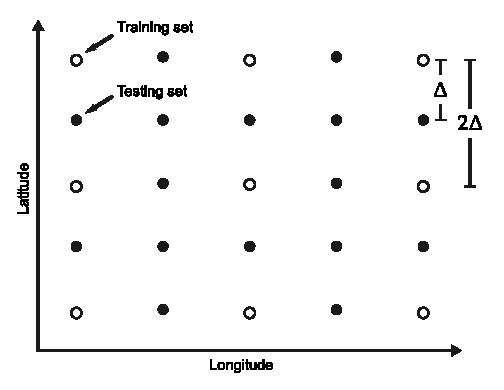
\includegraphics{figures/paper3/cv-grid-separation}
    \caption{Sketch of a data grid separated into
        the training (white dots with black outlines)
        and testing (black dots) data sets.
        The training data set is still displayed on a regular grid
        but with twice the grid spacing
        of the original data grid.}
    \label{fig:p3-grid_separation}
\end{figure}

The regularization parameter $\mu$ controls how much smoothness is applied to
the inversion result.
An optimal value of $\mu$ will stabilize and smooth the solution while not
compromising the fit to the observed data.
Two widely used methods to estimate an optimal $\mu$ are
the L-curve criterion and cross-validation \citep{hansen1992}.
Here, we will adopt the hold-out method of cross-validation \citep{kim2009}.
The hold-out method consists of splitting the observed data set into two
independent parts:
a training set $\mathbf{d}^o_{inv}$
and a testing set $\mathbf{d}^o_{test}$.
The training set is used in the inversion
while the testing set is kept back
and used to judge the quality of the chosen value of $\mu$.
For a value of the regularization parameter $\mu_k$,
the training set is inverted using $\mu_k$
to obtain an estimate $\mathbf{\hat{p}}^k$.
This estimate is used to calculate predicted data
on the same points as the testing set
via forward modeling
($\mathbf{d}_{test}^k = \mathbf{f}(\mathbf{\hat{p}}^k$)).
The metric chosen to evaluate $\mu_k$ is
the mean square error (MSE) of the misfit
between the observed and predicted testing data sets,

\begin{equation}
    MSE_k = \dfrac{\|\mathbf{d}^o_{test} - \mathbf{d}^k_{test}\|^2}{N_{test}},
    \label{eq:p3-msemu}
\end{equation}

\noindent
in which $N_{test}$ is the number of data in the testing set.
The optimal value of $\mu$ will be the one that minimizes the MSE,
i.e. the one that best predicts the testing data.
We emphasize that the inversion is performed only on the training data set.

The algorithm for the hold-out cross-validation is summarized as follows:

\begin{enumerate}
    \item Divide the observed data into
        the training ($\mathbf{d}^o_{inv}$)
        and testing ($\mathbf{d}^o_{test}$) sets.
    \item For each $\mu_k \in [\mu_1, \mu_2, \ldots, \mu_{N_{\mu}}]$:
    \begin{enumerate}
        \item Estimate $\mathbf{\hat{p}}^k$ by inverting the training set
            $\mathbf{d}^o_{inv}$.
        \item Use $\mathbf{\hat{p}}^k$ to calculate the predicted testing set
            $\mathbf{d}^k_{test}$.
        \item Calculate the mean square error $MSE_k$ using Eq.~\ref{eq:p3-msemu}.
    \end{enumerate}
    \item The final solution is the $\mathbf{\hat{p}}^k$ corresponding to the
        smallest $MSE_k$.
\end{enumerate}

The separation of the training and testing data sets is commonly done by taking
random samples from the full data set.
However, we cannot perform the separation in this way because
Bott's method requires data on a regular grid as well as having model elements
directly below each data point.
Thus, we take as our training set the points from the observed data grid that
fall on a similar grid but with twice the grid spacing
(white dots with black outlines in Fig.~\ref{fig:p3-grid_separation}).
All other points from the original data grid
make up the testing data set
(black dots in Fig.~\ref{fig:p3-grid_separation}).
This separation will lead to
a testing data set with more points than the training data set.
A way to balance this loss of data in the inversion
is to generate a data grid with half of the desired grid spacing,
either through interpolation
or from a spherical harmonic model.



%%%%%%%%%%%%%%%%%%%%%%%%%%%%%%%%%%%%%%%%%%%%%%%%%%%%%%%%%%%%%%%%%%%%%%%%%%%%%%%
\subsection{Estimating $z_{ref}$ and $\Delta\rho$}

The depth of the Normal Earth Moho ($z_{ref}$)
and the density-contrast of the anomalous Moho ($\Delta\rho$)
are other hyper-parameters of the inversion.
That is, their value influences the final solution
but they are not estimated during the inversion.
Both hyper-parameters cannot be determined from the gravity data alone.
Estimating $z_{ref}$ and $\Delta\rho$ requires
information that is independent of the gravity data,
such as knowledge of the parameters at certain points.
This information can be used in a manner similar to
the cross-validation described in the previous section.
In this study, we use point estimates of the Moho depth
to determine the optimal values of $z_{ref}$ and $\Delta\rho$.
These points will generally come from seismologic studies,
like receiver functions, surface wave dispersion, and deep refraction
experiments.

Let $\mathbf{z}_s^o$ be a vector of $N_s$ known Moho depths.
We use the mean square error (MSE)
as a measure of how well a given inversion output $\mathbf{\hat{p}}^k$
fits the know depths.
The optimal values of $z_{ref}$ and $\Delta\rho$
are the ones that best fit the independent known Moho depths
(i.e., produce the smallest MSE).
However, the points do not necessarily coincide
with the model elements of the inversion.
Before computing the MSE,
we interpolate $\mathbf{\hat{p}}^k$ on the known points
to obtain the predicted depths $\mathbf{z}_s^k$.
The MSE is defined as

\begin{equation}
    MSE = \dfrac{\|\mathbf{z}^o_s - \mathbf{z}^k_{s}\|^2}{N_s}.
    \label{eq:p3-msehyper}
\end{equation}

The algorithm for estimating $z_{ref}$ and $\Delta\rho$ is:

\begin{enumerate}
    \item For every combination of
        $z_{ref,l} \in [z_{ref,1},z_{ref,2},\ldots,z_{ref,N_z}]$ and
        $\Delta\rho_m \in
         [\Delta\rho_1,\Delta\rho_2,\ldots,\Delta\rho_{N_{\rho}}]$:
    \begin{enumerate}
        \item Perform the inversion on the training data set
            $\mathbf{d}^o_{inv}$ using $z_{ref,l}$, $\Delta\rho_m$, and
            the previously estimated value of $\mu$.
            The inversion output is the vector $\mathbf{\hat{p}}^{l,m}$.
        \item Interpolate $\mathbf{\hat{p}}^{l,m}$
            on the known points to obtain the predicted depths
            $\mathbf{z}_s^{l,m}$.
        \item Calculate the MSE between $\mathbf{z}_s^o$ and
            $\mathbf{z}_s^{l,m}$ using Eq.~\ref{eq:p3-msehyper}.
    \end{enumerate}
    \item The final solution is the $\mathbf{\hat{p}}^{l,m}$ corresponding to
        the smallest MSE.
\end{enumerate}

A similar approach was used by \citet{silva2006} and \citet{martins2010}
to estimate the parameters defining
the density-contrast variation with depth
of a sedimentary basin.
\citet{vandermeijde2013} also had
a similar methodology for dealing with the hyper-parameters,
though in a less formalized way.



%%%%%%%%%%%%%%%%%%%%%%%%%%%%%%%%%%%%%%%%%%%%%%%%%%%%%%%%%%%%%%%%%%%%%%%%%%%%%%%
\subsection{Software implementation}\label{sec:p3-software}

The inversion method proposed here is implemented in the Python programming
language.
The software is freely available
under the terms of the BSD 3-clause open-source software license.
Our implementation relies on the open-source libraries
scipy and numpy \citep[][ \url{http://scipy.org}]{jones2001}
for array-based computations,
matplotlib \citep[][ \url{http://matplotlib.org}]{hunter2007}
and seaborn
\citep[][ \url{http://stanford.edu/~mwaskom/software/seaborn}]{waskom2015}
for plots and maps,
and Fatiando a Terra \citep[][ \url{http://www.fatiando.org}]{uieda2013a}
for geophysics specific tasks,
particularly for forward modeling using tesseroids.
We use the scipy.sparse package for sparse matrix arithmetic and linear
algebra.
The sparse linear system in Eq.~\ref{eq:p3-gaussnewton-regul}
is solved using the conjugate gradient method implemented in scipy.sparse.

The computational experiments
(e.g., data processing, synthetic tests, real data application)
were performed in
Jupyter (formerly IPython) notebooks
\citep[][ \url{http://jupyter.org/}]{perez2007}.
The notebook files combine the source code used to run the experiments,
the results and figures generated by the code,
and rich text to explain and document the analysis.

All source code, Jupyter notebooks, data, and results
can be found at the online repository
\url{https://github.com/pinga-lab/paper-moho-inversion-tesseroids}.
The repository also contains instructions for replicating all results presented
here.
An archived version of this repository is also available at
\url{http://dx.doi.org/...}
(\textbf{Note to reviewers: the archived version will be uploaded upon
publication}).


%%%%%%%%%%%%%%%%%%%%%%%%%%%%%%%%%%%%%%%%%%%%%%%%%%%%%%%%%%%%%%%%%%%%%%%%%%%%%%%
\section{Application to synthetic data}

We test and illustrate the proposed inversion method
by applying it to two noise-corrupted synthetic data sets.
The first data set is generated by a simple Moho model simulating the transition
from a thicker continental crust to a thinner oceanic crust.
This application uses cross-validation to estimate the regularizing parameter
($\mu$) while assuming that the anomalous Moho density-contrast ($\Delta\rho$)
and the Normal Earth Moho depth ($z_{ref}$) are known quantities.
This first test is simplified in order to investigate solely
the efficiency of the inversion and
the cross-validation procedure to estimate $\mu$.
The second data set is generated by a more complex model derived from
the South American portion of the global CRUST1.0 model \citep{laske2013}.
This application uses cross-validation to estimate all three hyper-parameters:
$\mu$, $\Delta\rho$, and $z_{ref}$.
The model and corresponding synthetic data are meant to simulate
with more fidelity the real data application.


%%%%%%%%%%%%%%%%%%%%%%%%%%%%%%%%%%%%%%%%%%%%%%%%%%%%%%%%%%%%%%%%%%%%%%%%%%%%%%%
\subsection{Simple model}\label{sec:p3-simple-synthetic}

\begin{figure}
    \centering
    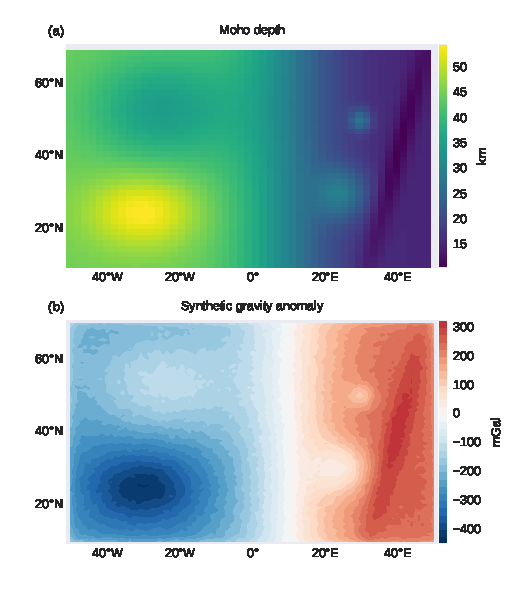
\includegraphics{figures/paper3/synthetic-simple-data}
    \caption{
        A simple Moho model made of tesseroids for synthetic data application.
        (a) The Moho depth of the model in kilometers.
        The model transitions from a deep Moho in the right to a shallow Moho in
        left, simulating the transition between a continental and an oceanic
        Moho.
        Each pixel in the pseudo-color image corresponds to a tesseroid of the
        model.
        (b) Noise-corrupted synthetic gravity data generated from the model
        shown in (a).
    }
    \label{fig:p3-simple-data}
\end{figure}

\begin{figure*}
    \centering
    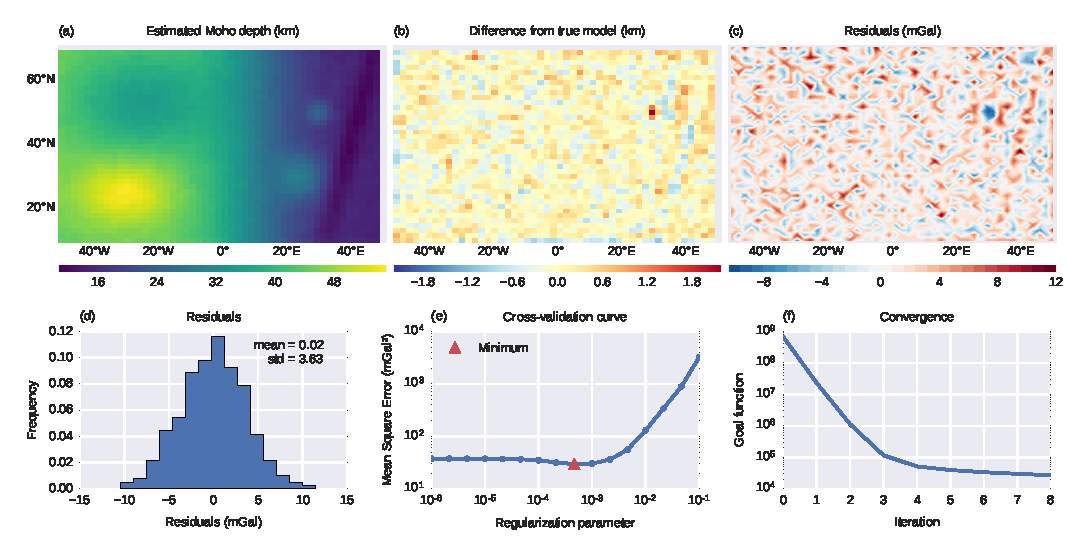
\includegraphics[width=\textwidth]{figures/paper3/synthetic-simple-results}
    \caption{
        Results from the inversion of the simple synthetic data.
        (a) The estimated Moho depth.
        (b) The difference between the true model depths
        and the estimated depths.
        (c) The inversion residuals (observed data minus
        the data predicted by the estimate).
        (d) Histogram of the residuals. Also shown are the calculated
        mean and standard deviation (std) of the residuals.
        Note that the data were contaminated with normally distributed
        pseudo-random noise with zero mean and 5 mGal standard deviation.
        (e) Cross-validation curve used to determine the optimal regularization
        parameter (Eq.~\ref{eq:p3-goalfunction}).
        Both axis are in logarithmic scale.
        The minimum Mean Square Error (Eq.~\ref{eq:p3-msemu}) is found at
        $\mu = 0.00046$ (red triangle).
        (f) Goal function value (Eq.~\ref{eq:p3-goalfunction}) per Gauss-Newton
        iteration showing the convergence of the gradient descent.
        The y-axis is in logarithmic scale.
    }
    \label{fig:p3-simple-results}
\end{figure*}

We simulate the transition from a continental-type Moho to an oceanic-type Moho
using a model composed of $M_{lat} \times M_{lon} = 40 \times 50$ grid of
juxtaposed tesseroids (a total of $M = 2000$ model elements).
The anomalous Moho density-contrast is $\Delta\rho = 400\ kg/m^3$
and the Normal Earth Moho depth is $z_{ref} = 30\ km$.
Fig.~\ref{fig:p3-simple-data}a shows the model Moho depths,
where each pixel in the pseudo-color image corresponds to
a tesseroid of the model.

The synthetic data were forward modeled on a regular grid of
$N_{lat} \times N_{lon} = 79 \times 99$ points
(a total of $N = 7821$ observations)
at a constant height of 50 km.
The data were contaminated with pseudo-random noise
sampled from a normal distribution with zero mean and 5 mGal standard deviation.
Fig.~\ref{fig:p3-simple-data}b shows the noise-corrupted full synthetic data set.
The data grid spacing is half the grid spacing of the tesseroid model
so that, when separating the training and testing data sets
(Fig.~\ref{fig:p3-grid_separation}),
the training data set points will fall directly above each model element.

We separated the synthetic data into training and testing data sets
following Fig.~\ref{fig:p3-grid_separation}.
The training data set is a regular grid of
$N_{lat} \times N_{lon} = 40 \times 50$ points
(a total of $N_{train} = 2000$).
The testing data set is composed of $N_{test} = 5821$ observations.
We used cross-validation to estimate an optimal regularization parameter ($\mu$)
from a set of $N_\mu = 16$ values equally spaced on a logarithmic scale
between $10^{-6}$ and $10^{-1}$.
We ran our regularized inversion on the training data set
for each value of $\mu$,
obtaining 16 Moho depth estimates.
For all inversions, the initial Moho depth estimate
used to start the Gauss-Newton optimization
was set to 60 km depth for all inversion parameters.
Furthermore, $z_{ref}$ and $\Delta\rho$ are set to their respective true values.
Finally, we computed the mean square error (MSE, Eq.~\ref{eq:p3-msemu})
for each estimate and chose as the final estimated Moho model
the one that minimizes the MSE.

Fig.~\ref{fig:p3-simple-results} summarizes the inversion results.
Fig.~\ref{fig:p3-simple-results}a shows the final estimated Moho depth
after cross-validation.
The recovered model is smooth, indicating that the cross-validation procedure
was effective in estimating an optimal regularization parameter.
Fig.~\ref{fig:p3-simple-results}b shows difference between the true Moho depth
(Fig.~\ref{fig:p3-simple-data}a) and the estimated Moho depth.
The differences appear to be semi-randomly distributed with a maximum
coinciding with a short-wavelength feature in the true model.
The maximum and minimum differences are approximately
2.19 and -2.13 km, respectively.
Fig.~\ref{fig:p3-simple-results}c shows inversion residuals (difference between
the observed and predicted data), in mGal.
The largest residual (in absolute value) coincides with the largest difference
between the true model and the estimate.
The inversion residuals are normally distributed,
as shown in Fig.~\ref{fig:p3-simple-results}d,
with 0.02 mGal mean and a standard deviation of 3.63 mGal.
The cross-validation curve in Fig.~\ref{fig:p3-simple-results}e
shows a clear minimum MSE at $\mu = 0.00046$
(indicated by the red triangle).
Fig.~\ref{fig:p3-simple-results}f shows the convergence of
the Gauss-Newton optimization in eight iterations.

We also investigated the computation time spent in each section of the inversion
process using a source code profiler.
The profiler measures how much time is spent inside each function during
the execution of a program.
We ran the profiler on a single inversion of the training data set
using the estimated regularization parameter.
We tracked the total time spent inside each of the three functions
that represent the largest computational bottlenecks of the inversion:
solving the linear system in Eq.~\ref{eq:p3-gaussnewton-regul}
using the conjugate gradient method,
performing the dot products required to compute
the Hessian matrix (Eq.~\ref{eq:p3-hessian-regul})
and the gradient vector (Eq.~\ref{eq:p3-gradient-regul}),
and forward modeling to calculate the predicted data (Eq.~\ref{eq:p3-forward}).
The profiling results presented in Table~\ref{profiling}
show that the time spent on forward modeling accounts for approximately
99.8\% of the total computation time.


\begin{table}
    \centering
    \caption{
        Total time spent on each function during a single inversion of
        simple synthetic data.
        The inversion was performed on a laptop computer with a
        Intel(R) Core(TM) i7-3612QM CPU @ 2.10GHz processor.
        The total time for the inversion was 42.133 seconds.
    }
    \label{profiling}
    \begin{tabular}{lcc}
        Function description & Time & Percentage of total time\\
        \hline
        Sparse conjugate gradient & 0.021 s & 0.050\%\\
        Sparse dot product & 0.007 s & 0.017\%\\
        Tesseroid forward modeling & 42.059 s & 99.824\%\\
        \hline
    \end{tabular}
\end{table}



%%%%%%%%%%%%%%%%%%%%%%%%%%%%%%%%%%%%%%%%%%%%%%%%%%%%%%%%%%%%%%%%%%%%%%%%%%%%%%%
\subsection{Model based on CRUST1.0}\label{sec:p3-crust1}

\begin{figure*}
    \centering
    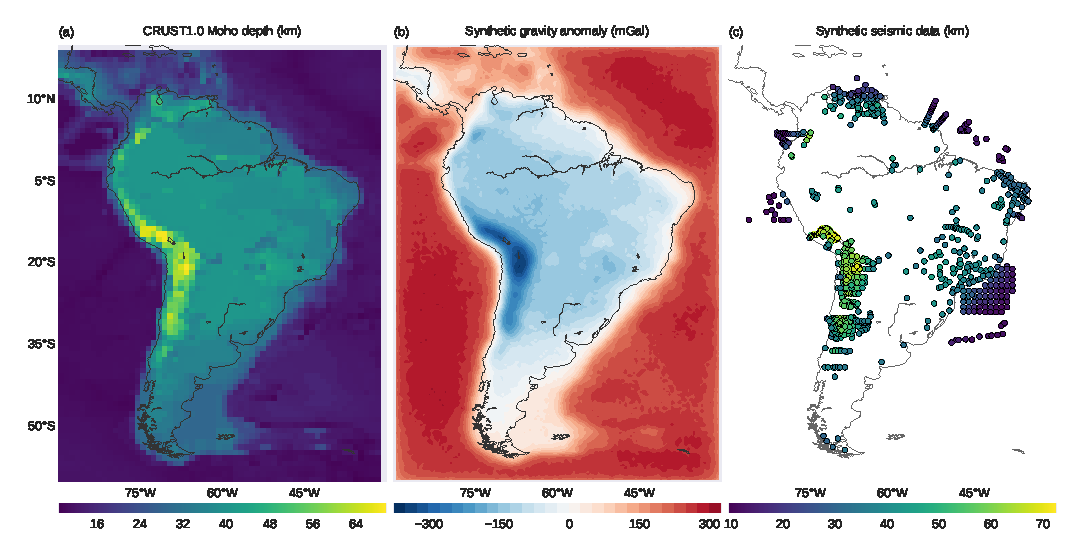
\includegraphics[width=\textwidth]{figures/paper3/synthetic-crust1-data}
    \caption{
        Synthetic data of a model derived from CRUST1.0.
        The model is made of tesseroids with an constant density-contrast
        of $\Delta\rho = 350\ kg/m^3$ and assuming a reference level of
        $z_{ref} = 30\ km$.
        (a) The Moho depth of the model in kilometers.
        Each pixel in the pseudo-color image corresponds to a tesseroid of the
        model.
        (b) Noise-corrupted synthetic gravity data generated from the model.
        (c) Synthetic seismic data simulating point estimates of Moho depth.
        The point estimates were obtained by interpolating
        the Moho depth in (a).
    }
    \label{fig:p3-crust1-data}
\end{figure*}

\begin{figure*}
    \centering
    \includegraphics[width=\textwidth]{figures/paper3/synthetic-crust1-results}
    \caption{
        Inversion results from the CRUST1.0 synthetic data.
        (a) Cross-validation curve used to determine
        the regularization parameter (Eq.~\ref{eq:p3-goalfunction}).
        The minimum Mean Square Error (Eq.~\ref{eq:p3-msemu}) is found at
        $\mu = 0.0001$ (red triangle).
        (b) Cross-validation results used to determine
        the reference level ($z_{ref}$) and the density-contrast ($\Delta\rho$).
        The colored contours represent
        the Mean Square Error (Eq.~\ref{eq:p3-msehyper}) in $km^2$.
        The minimum (red triangle) is found at $z_{ref} = 30\ km$
        and $\Delta\rho = 350\ kg/m^3$.
        (c) The estimated Moho depth.
        (d) Difference between the CRUST1.0 model depths
        (Fig.~\ref{fig:p3-crust1-data}a)
        and the estimated depths.
        (e) Histogram of the inversion residuals
        (observed minus predicted data).
        (f) Histogram of the differences between
        the synthetic seismic observations (Fig.~\ref{fig:p3-crust1-data}c)
        and the estimated depths.
        (g) The inversion residuals.
        (h) Difference between the seismic and the estimated depths.
    }
    \label{fig:p3-crust1-results}
\end{figure*}


In this test, we simulate the anomalous Moho of South America
using Moho depth information extracted from the CRUST1.0 model
\citep{laske2013}.
We construct a tesseroid model with
$M_{lat} \times M_{lon} = 80 \times 60$ juxtaposed elements, 4800 in total,
using the Moho depths shown in Fig.~\ref{fig:p3-crust1-data}a.
In our model, the Normal Earth Moho is $z_{ref} = 30\ km$ and
the density-contrast is $\Delta\rho = 350\ kg/m^3$.
We produce the synthetic data at a constant height of 50 km
and on a regular grid of $N_{lat} \times N_{lon} = 159 \times 119$ points
(a total of 18921 observations).
We contaminate the synthetic data with normally distributed pseudo-random noise
with zero mean and 5 mGal standard deviation (Fig.~\ref{fig:p3-crust1-data}b).

The cross-validation procedure to determine $\Delta\rho$ and $z_{ref}$
requires knowledge of the Moho depth at certain points
($\mathbf{z}_s^o$ in Eq.~\ref{eq:p3-msehyper}),
usually from seismic experiments.
Thus, we must also generate synthetic seismic data about the Moho depth.
We produce such data by interpolating the Moho depth shown in
Fig.~\ref{fig:p3-crust1-data}a on the same geographic coordinates
as the 937 points from the \citet{assumpcao2013a} data set.
The resulting synthetic seismic data is shown in Fig.~\ref{fig:p3-crust1-data}c.

We perform the cross-validation procedures in two parts.
First, we run the cross-validation to estimate
an optimal regularization parameter ($\mu$).
The starting estimate for all inversions is
60 km depth for all model parameters.
For this cross-validation,
we keep $z_{ref}$ and $\Delta\rho$ fixed to
$20\ km$ and $500\ kg/m^3$, respectively.
Our investigations suggest that the outcome of this round of cross-validation
does not depend on the particular values of $z_{ref}$ and $\Delta\rho$ used.
Second, we use the estimated $\mu$ to run the cross-validation
to estimate $z_{ref}$ and $\Delta\rho$,
thus obtaining the final estimated Moho depths.
Fig.~\ref{fig:p3-crust1-results} summarizes the results
from both cross-validation runs and the final inversion results.

For the first cross-validation,
we separate the synthetic data (Fig.~\ref{fig:p3-grid_separation}) into
a training set with twice the grid spacing of the original data
($N_{lat} \times N_{lon} = 80 \times 60$)
and a testing set with 14,121 observations.
We run the inversion for 16 different values of $\mu$
equally spaced in a logarithmic scale between $10^{-7}$ and $10^{-2}$.
For each of the 16 estimates we compute the MSE (Eq.~\ref{eq:p3-msemu}),
shown in Fig.~\ref{fig:p3-crust1-results}a as function of $\mu$.
The optimal regularization parameter that minimizes the MSE is $\mu = 10^{-4}$
(indicated by the red triangle).

In the second cross-validation,
we use the estimated value of $\mu$ in all inversions.
We test seven values of $z_{ref}$ from 20 to 35 km with 2.5 km intervals
and seven values of $\Delta\rho$ from 200 to 500 $kg/m^3$
with 50 $kg/m^3$ intervals.
We run the inversion for every combination of $z_{ref}$ and $\Delta\rho$,
totaling 49 inversions.
Finally, we calculate the Mean Square Error (Eq.~\ref{eq:p3-msehyper})
for each of the 49 estimates
and choose the values of $z_{ref}$ and $\Delta\rho$ that minimize the MSE.
Fig.~\ref{fig:p3-crust1-results}b
shows a colored-contour map of the MSE
with a minimum (marked by the red triangle)
at $z_{ref} = 30\ km$ and $\Delta\rho = 350\ kg/m^3$.

Fig.~\ref{fig:p3-crust1-results}c shows the final solution after both
cross-validation procedures.
The recovered model is smooth, indicating that the cross-validation procedure
was effective in estimating an optimal regularization parameter.
Fig.~\ref{fig:p3-crust1-results}d shows the difference between
the true Moho depths (Fig.~\ref{fig:p3-crust1-data}a)
and the estimated depths.
The maximum and minimum differences are, respectively,
9.8 and -8.2 km.
The largest absolute differences are located along the central and northern
Andes, where there is a sharp increase in the true Moho depth
(Fig.~\ref{fig:p3-crust1-data}a).
Positive differences (indicating a too shallow estimate)
appear along the central portion of the Andes,
flanked by regions of negative differences (indicating a too deep estimate)
on the continental and Pacific sides.
Figs.~\ref{fig:p3-crust1-results}e and g show the inversion residuals (difference
between the observed and predicted data).
The inversion residuals appear normally distributed,
with 0.03 mGal mean and a standard deviation of 4.10 mGal.
The residuals follow a similar, though reversed, pattern
to the differences shown in Fig.~\ref{fig:p3-crust1-results}d.
The largest residuals (in absolute value) are along the Andes,
with the central portion being dominated by negative residuals
and flanked by positive residuals on both sides.
Figs.~\ref{fig:p3-crust1-results}f and h show the differences between
the synthetic seismic data (Fig.~\ref{fig:p3-crust1-data}c)
and the estimated Moho depths.
Once more, the largest differences are concentrated along the Andes,
particularly in the central Andes and near Ecuador and Colombia.
The differences are smaller along the Atlantic coast of South America,
with notable larger differences in a few points of northeastern Brazil
and along the Amazon river.
In general, large residuals are associated with sharp increases in Moho depth.



%%%%%%%%%%%%%%%%%%%%%%%%%%%%%%%%%%%%%%%%%%%%%%%%%%%%%%%%%%%%%%%%%%%%%%%%%%%%%%%
\section{Application to the South American Moho}


We apply the inversion method proposed here to invert for the Moho depth of the
South American continent.
We follow the application of \citet{vandermeijde2013} but with some
differences, mainly using a different data set and performing all modeling
in spherical coordinates using tesseroids.
The data are corrected of the effects of topography and sedimentary basins.
Crust and mantle heterogeneities cannot be properly accounted for
in regions where information coverage is sparse and readily accessible models
are not available, like in South America and Africa.
Hence, for the purposes of this study, we will assume to be negligible all
other crustal and mantle sources, including lateral variations in density along
the Moho.


%%%%%%%%%%%%%%%%%%%%%%%%%%%%%%%%%%%%%%%%%%%%%%%%%%%%%%%%%%%%%%%%%%%%%%%%%%%%%%%
\subsection{Gravity and seismic data}

\begin{figure*}
    \centering
    \includegraphics[width=\textwidth]{figures/paper3/south-america-corrections}
    \caption{
        Gravity data for South America and the models used in the data
        corrections.
        (a) The gravity disturbance (Eq.~\ref{eq:p3-disturbance}) calculated from
        the raw gravity data.
        (b) Topography from ETOPO1.
        (c) Gravitational attraction of the topography calculated
        at the observation height using tesseroids.
        (d) The Bouguer disturbance (Eq.~\ref{eq:p3-bouguer}) obtained by
        subtracting (c) from (a).
        The upper (e), middle (f), and lower (g) sediment layer thicknesses
        from the CRUST1.0 model.
        (h) The total gravitational attraction of the sediment layers shown in
        (e), (f), and (g), calculated using tesseroids.
        }
    \label{fig:p3-sam-corrections}
\end{figure*}

\begin{figure*}
    \centering
    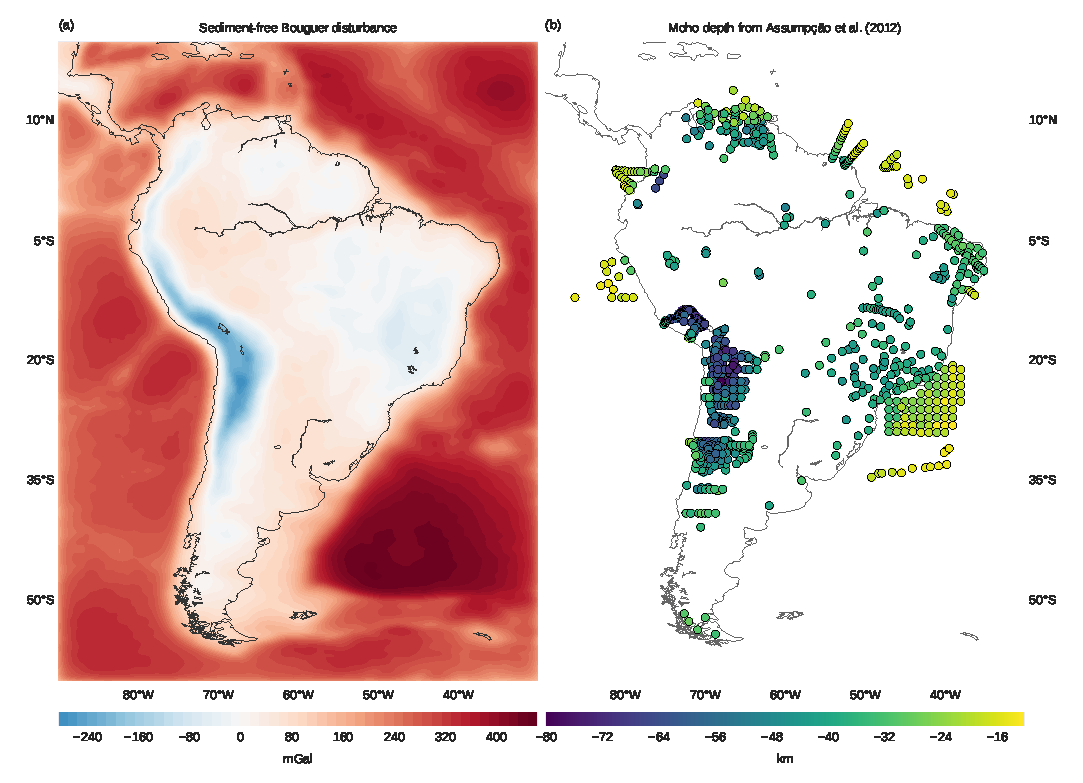
\includegraphics[width=\textwidth]{figures/paper3/south-america-data}
    \caption{
        Input data for the South American Moho inversion.
        (a) Sediment-free Bouguer disturbance for South America.
        Obtained by subtracting the total sediment gravitational effect
        (Fig.~\ref{fig:p3-sam-corrections}h) from the Bouguer disturbance
        (Fig.~\ref{fig:p3-sam-corrections}d).
        (b) Seismological Moho depth estimates from
        \citet{assumpcao2013a}.
    }
    \label{fig:p3-sam-data}
\end{figure*}


The raw gravity data are generated from the satellite only
spherical harmonic model GOCO5S \citet{mayer-guerr2015}.
The GOCO5S model combines data from 15 satellites, including the complete
mission data from the GOCE satellite.
The data were downloaded from the
International Centre for Global Earth Models (ICGEM) web-service
\citep[][ \url{http://icgem.gfz-potsdam.de/ICGEM/})]{barthelmes2012}
in the form of the complete gravity field
on a regular grid with $0.2^\circ$ grid spacing at ellipsoidal height 50 km.
We calculate the gravity disturbance
($\delta(P)$ in Eq.~\ref{eq:p3-disturbance})
by subtracting from the raw data
the normal gravity of the WGS84 reference ellipsoid ($\gamma(P)$)
using the formula of \citet{li2001a}.
Fig.~\ref{fig:p3-sam-corrections}a show the calculated gravity disturbance of
South America.

We remove the gravitational effect of the topography
from the gravity disturbance
by modeling the ETOPO1 digital terrain model
\citep[][ \url{http://dx.doi.org/10.7289/V5C8276M}]{amante2009}
using tesseroids (Fig.~\ref{fig:p3-sam-corrections}b).
We used the standard densities of $2670\ kg/m^3$ for continents and
$-1630\ kg/m^3$ for the oceans.
Fig.~\ref{fig:p3-sam-corrections}c shows the calculated gravitational attraction
of the topographic masses at 50 km height.
Fig.~\ref{fig:p3-sam-corrections}d shows the Bouguer disturbance
(Eq.~\ref{eq:p3-bouguer}) obtained after subtracting the topographic effect from
the gravity disturbance.

The effect of sedimentary basins is removed using
tesseroid models of the three sedimentary layers present in the CRUST1.0 model
\citep[][ \url{http://igppweb.ucsd.edu/~gabi/rem.html}]{laske2013}.
Each sedimentary layer model includes the density
of each $1^\circ \times 1^\circ$ model cell.
Figs.~\ref{fig:p3-sam-corrections}e-g show the thickness of the upper, middle, and
lower sedimentary layers, respectively.
The density-contrasts of the tesseroid model is obtained by subtracting
$2670\ kg/m^3$ from the density of each model element.
Fig.~\ref{fig:p3-sam-corrections}h shows the combined gravitational attraction of
the sedimentary basin tesseroid model.
We subtract the total effect of sediments from the Bouguer disturbance in
Fig.~\ref{fig:p3-sam-corrections}d to obtain
the sediment-free Bouguer disturbance (Fig.~\ref{fig:p3-sam-data}a),
which will be used as input for the inversion.

The seismic point estimates of Moho depth used in the cross-validation
procedure are from the data set of \citet{assumpcao2013a}.
The 937 data points in this data set are shown in Fig.~\ref{fig:p3-sam-data}b.


%%%%%%%%%%%%%%%%%%%%%%%%%%%%%%%%%%%%%%%%%%%%%%%%%%%%%%%%%%%%%%%%%%%%%%%%%%%%%%%
\subsection{Inversion and cross-validation}

\begin{figure}
    \centering
    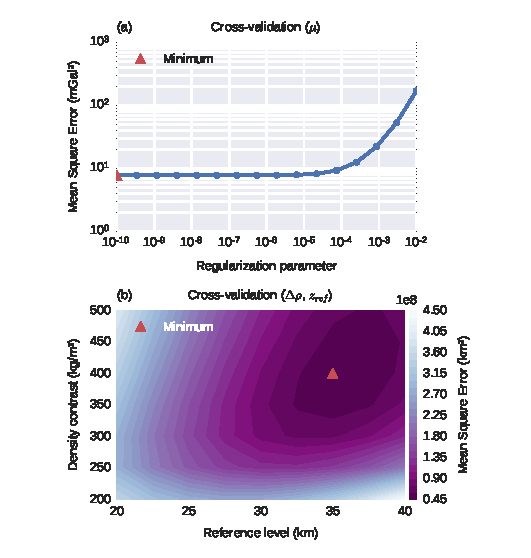
\includegraphics{figures/paper3/south-america-cv}
    \caption{
        Cross-validation results for the South American Moho inversion.
        (a) Cross-validation to determine the regularization parameter $\mu$
        (Eq.~\ref{eq:p3-goalfunction}).
        The minimum Mean Square Error (Eq.~\ref{eq:p3-msemu}),
        shown as a red triangle,
        corresponds to $\mu = 10^{-10}$.
        (b) Cross-validation to determine
        the reference level ($z_{ref}$) and the density-contrast ($\Delta\rho$).
        The colored contours represent
        the Mean Square Error (Eq.~\ref{eq:p3-msehyper}).
        The minimum (red triangle) is found at $z_{ref} = 35\ km$
        and $\Delta\rho = 400\ kg/m^3$.
    }
    \label{fig:p3-sam-cv}
\end{figure}



As in the CRUST1.0 synthetic data test (section~\ref{sec:p3-crust1}),
we perform the cross-validation in two parts.
First, we run the cross-validation to estimate
an optimal regularization parameter ($\mu$).
The starting estimate for all inversions is
60 km depth for all model parameters.
For this cross-validation,
we keep $z_{ref}$ and $\Delta\rho$ fixed to
$20\ km$ and $500\ kg/m^3$, respectively.
Second, we use the estimated $\mu$ to run the cross-validation
to estimate $z_{ref}$ and $\Delta\rho$,
thus obtaining the final estimated Moho depth model.

We split the sediment-free gravity data into the training and testing data
sets.
The training data set is a regular grid with $0.4^\circ$ grid spacing
(twice the spacing of the original data grid)
and $N_{lat} \times N_{lon} = 201 \times 151$ grid points,
a total of 30,351 observations.
The remaining 90,350 points compose the testing data set.
We test 16 values of the regularization parameter ($\mu$)
equally spaced on a logarithmic scale between $10^{-10}$ and $10^{-2}$.
Fig.~\ref{fig:p3-sam-cv}a shows the Mean Square Error (MSE)
as a function of $\mu$.
The minimum MSE is found at $\mu = 10^{-10}$, the lowest value of $\mu$ tested,
suggesting that little or no regularization is required.

We proceed with the second cross-validation using $\mu = 10^{-10}$ in all
inversions.
We test all combinations of
seven values of $z_{ref}$, from 20 to 35 km with 2.5 km intervals,
and seven values of $\Delta\rho$, from 200 to 500 $kg/m^3$
with 50 $kg/m^3$ intervals.
Fig.~\ref{fig:p3-sam-cv}b shows a map of the MSE
with respect to the \citet{assumpcao2013a} data set.
The MSE has a well defined minimum, indicated by the red triangle,
at $z_{ref} = 35\ km$ and $\Delta\rho = 400\ kg/m^3$.


%%%%%%%%%%%%%%%%%%%%%%%%%%%%%%%%%%%%%%%%%%%%%%%%%%%%%%%%%%%%%%%%%%%%%%%%%%%%%%%
\subsection{Moho model for South America}

\begin{figure*}
    \centering
    \includegraphics[width=\textwidth]{figures/paper3/south-america-moho}
    \caption{
        Inversion results for the South American Moho.
        (a) The estimated Moho depth of South America.
        The solid light grey line is the 35 km Moho depth contour.
        (b) Inversion residuals (observed data in Fig.~\ref{fig:p3-sam-data}a
        minus the data predicted by the estimate (a)).
        (c) Differences between the seismological depths of
        \citet{assumpcao2013a} and our gravity-derived estimate shown in (a).
        The inset in (c) shows a histogram of the differences along with their
        calculated mean and standard deviation (std).
    }
    \label{fig:p3-sam-moho}
\end{figure*}


The final Moho depth model for South America is shown
as a pseudo-color map in Fig.~\ref{fig:p3-sam-moho}a.
The model is available in the online repository that accompanies
this contribution (see section~\ref{sec:p3-software}).
Each model element is a $0.4^\circ \times 0.4^\circ$ tesseroid,
represented by the pixels in the pseudo-color map.

Our model differs significantly from CRUST1.0 (Fig.~\ref{fig:p3-crust1-data}a)
but contains most of the large-scale features
present in the GMSA12 gravity-derived model of \citet{vandermeijde2013}.
The deepest Moho is along the central Andes, reaching depths upward of 70 km.
The oceanic areas present the shallowest Moho, ranging approximately
from 7.5 to 20 km.
The Brazilian and Guiana shields have a deeper Moho (greater than 35 km),
with the deepest portion in the area of the São Francisco craton.
The Moho is shallower than 35 km along the western Amazon and Andean foreland
regions, as well as along the Amazon river.

Fig.~\ref{fig:p3-sam-moho}b shows the inversion residuals
(observed minus predicted data)
and Fig.~\ref{fig:p3-sam-moho}c shows the differences between
the seismic-derived depths of \citet{assumpcao2013a}
(Fig.~\ref{fig:p3-sam-data}b) and the depths in our model.
The differences range from approximately -23 to 23 km
and have a mean of 1.18 km and a standard deviation of 6.84 km.
The residuals and differences from seismic are smallest in the oceanic areas,
southern Patagonia, and the eastern coast of the continent.
The largest residuals are located along the Andes and correlate with the
deepest Moho depths.
These large residuals follow a pattern of a negative value in the center
flanked by positive values to the East and West.
This same pattern is observed in the CRUST1.0 synthetic test results
(Fig.~\ref{fig:p3-crust1-results}),
suggesting that this is a byproduct of the inversion method, not the data.
Likewise, larger residuals also appear to be associated with sharp variations
in the estimated Moho depth.
Along the Andes, large differences with seismic data are correlated with the
large inversion residuals.
Conversely, this correlation is absent from the large differences seen in
points around Venezuela.
In the Borborema province, northeastern Brazil,
our model slightly overestimates the Moho depth.
On the other hand, our model underestimates the depths
in the Amazon region and the Paraná basin.
Particularly in the Amazon basin,
where our model predicts a Moho depth of approximately 30 km,
the residuals and the differences with the seismic data are larger than in the
Paraná basin.



%%%%%%%%%%%%%%%%%%%%%%%%%%%%%%%%%%%%%%%%%%%%%%%%%%%%%%%%%%%%%%%%%%%%%%%%%%%%%%%
\section{Conclusions}

We have developed a computationally efficient gravity inversion method in
spherical coordinates.
Our method extends the Gauss-Newton formulation of Bott's method
\citep{silva2014} to use tesseroids as model elements and smoothness
regularization.
We retain the computational efficiency of Bott's method by taking advantage of
the sparse nature of all matrices involved.
We employ two cross-validation techniques to estimate the hyper-parameters of
the inversion: the regularization parameter, the Moho density-contrast, and the
Normal Earth Moho depth.

The test on simple synthetic data shows that our inversion method is able to
recover a smooth Moho relief with a homogeneous density-contrast.
The inversion was not able to fully recover the shortest wavelength feature in
the model, possibly due to the smoothness constraints which tends to soften
high-frequency (sharp) variations.
The cross-validation Mean Square Error curve in Fig.~\ref{fig:p3-simple-results}e
has a well-defined minimum, indicating a value of the regularization parameter
($\mu$) whose corresponding estimate best predicts data that were not included
in the inversion.
Using this value of $\mu$ in the inversion leads to a smooth Moho relief and
acceptable data misfit.

The source code profiling results presented in Table~\ref{profiling}
confirm the efficiency of the proposed method.
When using sparse matrices, solving linear systems and performing matrix
multiplications together account for a mere 0.067\% of the total computation
time required for a single inversion.
The majority of the computation time (99.824\%) is spent on forward modeling.
Thus, we are able to retain the high computational efficiency of Bott's method
while using a classic Tikhonov regularization formulation.
This approach could, in theory, be extended to other types of regularization
(e.g., Total Variation) and misfit functions (e.g., re-weighted least squares)
already available in the literature.
For example, the Total Variation approach used by \citet{martins2011} could
potentially be implemented in a more straight forward manner than done by
\citet{santos2015}.

The more complex synthetic data test based on CRUST1.0
(Fig.~\ref{fig:p3-crust1-results})
shows that the cross-validation using pointwise Moho depth information
is able to correctly estimate the density-contrast ($\Delta\rho$) and Normal
Earth Moho depth ($z_{ref}$).
This test indicates that the inversion neither correctly estimates Moho depth
nor adequately fits the gravity and pointwise data when sharp variations in
Moho depth occur.
This phenomenon is particularly strong in the region below the Andes.
A likely explanation is that the smoothness regularization
is intrinsically unable to produce sharp variations in Moho depth.
These effects might be mitigated with the use of sharpness-inducing
regularization, like Total Variation \citep{martins2011},
Cauchy norm regularization \citep{sacchi1996, pilkington2008},
or an adaptive mixed smoothness-sharpness regularization \citep{sun2014}.

We applied the method proposed here to estimate the Moho depth for South
America.
Our Moho depth model is in accordance with previous results by
\citet{vandermeijde2013}.
The model fits well the gravity and seismic data in all oceanic regions, the
central portion of the Andean foreland, Patagonia, and coastal and central
parts of Brazil.
However, the model is unable to fit the gravity and seismic data in places with
sharp variations in Moho depth, particularly below the Andes.
This might indicate the improper use of smoothness regularization, as suggested
by the CRUST1.0 synthetic data test, or the presence of crustal or mantle
density anomalies that were unaccounted for during the data corrections.
In the coastal region of Venezuela, along the central Amazon and Solimões
basins, and in the Paraná basin, the model is able to fit the gravity data but
differs significantly from the seismic data.
\citet{mariani2013} and \citet{nunn1988} explain these discrepancies in the
Paraná and Amazon basins, respectively, as high density rocks in the lower
crust.
In general, differences between a gravity and a seismically derived Moho model
may indicate the presence of crustal or mantle density anomalies that were
unaccounted for in the data processing.
Such locations warrant further detailed investigation.



%%%%%%%%%%%%%%%%%%%%%%%%%%%%%%%%%%%%%%%%%%%%%%%%%%%%%%%%%%%%%%%%%%%%%%%%%%%%%%%
\section{Acknowledgments}

We are indebted to the developers and maintainers of the open-source
software without which this work would not have been possible.
L. Uieda was supported by a scholarship from
Coordenação de Aperfeiçoamento de Pessoal de Nível Superior
(CAPES).
V.C.F. Barbosa was supported by a fellowship from
Conselho Nacional de Desenvolvimento Científico e Tecnológico (CNPq).

\chapter{Conclusions}


We have developed two open-source software packages that implement the
components required for building an inversion method: forward modeling,
optimization, and regularization.
We used these components to develop a fast gravity inversion method to estimate
the depth of the crust-mantle interface (the Moho) in a spherical
approximation.
We then applied the proposed method to estimate the Moho depth for South
America.

The \textit{Tesseroids} software is a collection of command-line
programs developed in the C programming language.
The programs calculate the gravitational potential and its first and second
derivatives of a tesseroid (spherical prism) model.
We implemented and improved upon an adaptive discretization algorithm to
guarantee the accuracy of the computations.
The adaptive discretization is controlled by a scalar called the distance-size
ratio ($D$).
Higher values of $D$ result in finner discretization and vice-versa.
Furthermore, we investigated the accuracy of the calculations as a function of
$D$.
Contrary to previous assumptions, our results showed that the first and second
derivatives require finner discretization than the gravitational potential to
achieve the same accuracy level.
The values of the distance-size ratio that yield a maximum error of 0.1\%
are $D = 1$ for the gravitational potential, $D = 1.5$ for the first
derivatives, and $D = 8$ for the second derivatives.
These values are included as defaults in version 1.2 of the \textit{Tesseroids}
software.

\textit{Fatiando a Terra} is a software library implemented in the Python
programming language.
The library contains functions and classes for data processing, visualization,
inversion, and forward modeling.
The inverse problems package of the library offers generic classes for
optimization and regularization.
These classes can be extended and combined with the existing forward modeling
functions to implement new inversion methods.
Using these tools, the amount of code required to implement a new method is
reduced, increasing the speed of the cycle of prototyping a new algorithm,
testing, and then refining it.
The project has been used in scholarly works such as
\citet{carlos2014}, \citet{hidalgo-gato2015a}, \citet{niccoli2015},
\citet{oliveirajr.2015}, and \citet{bassett2016}.
To date, the project has received contributions from nine developers in three
different countries.


\backmatter
\bibliographystyle{on-plain}
\bibliography{references}

\end{document}
